\section{Data-quality issues}
\label{sec:dataquality}

\subsection{Forward HCAL (HF) Noise}
\label{subsec:hfnoise}

The forward HCAL (HF) detector covers the most-forward rapidity range of HCAL ($3 < |\eta| < 5$), as described in
Sec.~\ref{subsec:hcal}. Due to its very forward location and close proximity to the beam pipe, 
HF detector operates in a much harsher radiation environment. 
It should also be noted that the tracking detector, covering $|\eta| < 2.5$ range, does not extend to this high rapidity
phase space. Combination of these different factors makes it harder to reconstruct and cluster hadronic jets, 
and measure their energies accurately at the HF detector. Therefore, there
is a sizable probability that the $\pt$ of a jet reconstructed at high $|\eta|$ being highly mismeasured.
Such mismeasurements can lead to spurious $\ptmiss$ in QCD multijet events (e.g. $q\bar{q} \rightarrow q\bar{q}$),
due to $\pt$ of one of the final state jets being severely mismeasured. It should be noted that while the probability
of such severe mismeasurement is relatively small, the very large cross section of QCD multijet processes in a p-p collider
compensates for this, and the number of events with spurious $\ptmiss$ cannot be ignored.
This becomes problematic for analyses that target $\ptmiss$ (such as analyses targeting $\hinv$ signature), 
since mismeasured QCD multijet events can pass
the high $\ptmiss$ requirement imposed on the analysis signal region. Hence, this effect needs to taken into account. 

It was observed that jets resulting from such mismeasurement present a distinguishable shape with respect to well-identified jets: 
Their shower shape is spread in $\eta$ and narrow in $\phi$. Shower shape variables of HF jets ($\sieie$, $\sipip$, HF central strip size) 
have therefore been introduced and added to the event content in the input datasets. 
$\sieie$ represents the shower width of the HF jet in $\eta$ direction, and similarly, $\sipip$ represents the shower width in $\phi$ direction. 
Their definitions can be found below:

\begin{equation}
    \begin{split}
        \sieie &= \sqrt{\frac{ \sum_{i} \Delta\eta(i, jet)^2 \omega_i }{ \sum_{i} \omega_i }} \\
        \sipip &= \sqrt{\frac{ \sum_{i} \Delta\phi(i, jet)^2 \omega_i }{ \sum_{i} \omega_i }}
    \end{split}
    \label{eq:sieie_sipip}
\end{equation}

In Eq.~\ref{eq:sieie_sipip}, the sums run over all PF candidates with $\pt > 3$ GeV, and 
$\omega_i$ is the weight applied to PF candidate $i$ within the jet, which is computed as follows:

\begin{equation}
    \omega_i = \frac{p_T^i - p_T^{\text{PU offset}}}{\sum_{i} p_T^{i} - p_T^{\text{PU offset}} }
    \label{eq:omega_def}
\end{equation}

In Eq.~\ref{eq:omega_def}, $p_T^{\text{PU offset}}$ refers to the offset correction on the $\pt$ of the particle 
due to pileup (PU). It is defined as follows:

\begin{equation}
    p_T^{\text{PU offset}} = \frac{\text{jet L1 offset / gen vtx}}{\pi \times 0.4^2} \times \frac{N_{\text{reco vertices}}}{\epsilon^{reco}(\text{PU vtx})} \times S_{\text{HF tower}}
\end{equation}

The other distinguishing variable, HF central strip size ($\hfcss$), is computed as follows: 
$N_{cands}$ with $\pt > 10$ GeV \& $|\Delta\phi(cand,jet)| < 0.05$. It is a measure of the number of
highly energetic particles reconstructed close to the jet centroid (i.e. $|\Delta\phi(cand,jet)| < 0.05$).
In the event of spurious large energy deposits from a jet, one can expect larger number of energetic particles
being reconstructed closer to the jet centroid, as a result of those energy deposits.

These variables are used to define a series of cuts rejecting most of the HF-related noise, while keeping a high efficiency on well-identified jets. 
The efficiency of the cuts on physics jets in data and simulation is measured and their ratio is used to correct the simulation.
This procedure is described in Sec.~\ref{subsec:hf_weighting}. After the HF noise cuts are applied, the residual noise in the signal region is estimated using a data driven technique.
The study and the definition of the HF noise cuts, and the residual HF noise estimation are discussed in the subsections below. 

\subsubsection{Definition of HF Noise Cuts}

In order to study the discriminating power of these variables directly in data, two regions enriched in ``physics'' jets and ``noise'' jets are defined. ``Physics'' jets
refer to HF jets that are recoiling against a well-reconstructed physics object (in this study, a photon), and ``noise'' jets 
refer to HF jets that recoil against no visible physics object, hence creating $\ptmiss$ in the event. The region where the ``physics'' jets are tagged
is termed as the physics-enriched region, and the region where the ``noise'' jets are tagged is termed as the noise-enriched region.

The physics-enriched region consists of events where a HF jet recoils against a photon. 
Jet and photon being back-to-back is ensured by a series of cuts on $\Delta\phi(\gamma, jet)$,
ratio of transverse momenta of the photon and the jet, and also the requirement of low $\ptmiss$ in the event. The selections are listed below: 

\begin{itemize}
    \item Exactly one well identified photon (tight identification, as discussed in Sec.~\ref{subsec:photons})
    \item Events passing a single photon trigger requiring $p_T^{\gamma} > 110$ GeV
    \item $\Delta\phi(\gamma, jet) > 2.7$
    \item $0.5 < \frac{p_T(\gamma)}{p_T(jet)} < 1.5$
    \item $\ptmiss < 50$ GeV
\end{itemize}

The noise-enriched region includes events with exactly one high $\pt$ HF jet and high $\ptmiss$.
The aim here is to collect events with a mis-measured HF jet, such that it has very high $\pt$, but there is no other high $\pt$ physics object in the event,
giving rise to $\ptmiss$ in the event.
The complete requirements for this region are listed below:

\begin{itemize}
    \item Events passing the MET trigger described in Sec.~\ref{subsubsec:met_trigger_eff}, requiring $\ptmiss > 120$ GeV and $\htmiss > 120$ GeV
    (as reconstructed by the trigger algorithm). 
    \item $\ptmiss > 100$ GeV
    \item Exactly one HF jet with $\pt > 100$ GeV
    \item No extra jet with $\pt > 30$ GeV
    \item No lepton with $\pt > 10$ GeV
\end{itemize}

The two regions outlined above are used to study the distribution of HF shower shape variables for well-identified jets, as opposed to events
containing a mis-measured (``noisy'') jet. Mainly, two sets of cuts are studied and adopted in the analysis:

\begin{itemize}
    \item Cuts on $\sieie$ and $\sipip$
    \item Cut on HF central strip size
\end{itemize}

Since the HF-related noise strongly peaks in the $3<|\eta|<3.25$ region and the size of the HF towers is $|\eta|$ dependent, 
possibly affecting the variables under study, three $|\eta|$ regions are considered. 
Two dimensional distributions of $\sipip$ vs  $\sieie$ are shown in Fig.~\ref{fig:sieie_sipip_noise_enriched} and Fig.~\ref{fig:sieie_sipip_physics_enriched},
for the noise and physics enriched regions respectively. 
From Fig.~\ref{fig:sieie_sipip_noise_enriched}, the skewness of the 2D distribution towards high $\sieie$ and low $\sipip$
can be observed, specifically for $|\eta| < 4$. This motivates the diagonal cut of $\sieie - \sipip < 0.02$, cutting away a sizable number of noisy events while
having much less impact in the physics-enriched region. 

In the noise enriched region, there are also a large number of events observed within the region defined by $\sieie < 0.02$ and $\sipip < 0.02$. 
These are thought to be interactions of halo muons in the HF detector and this region with very low $\sieie$ and $\sipip$ is therefore also vetoed. 

For jets with $|\eta| > 4$, the requirement becomes $\sieie < 0.1$ and $\sipip > 0.02$, as large numbers of noise events are observed at very low
$\sipip$ and high $\sieie$.

\begin{figure}
    \centering
    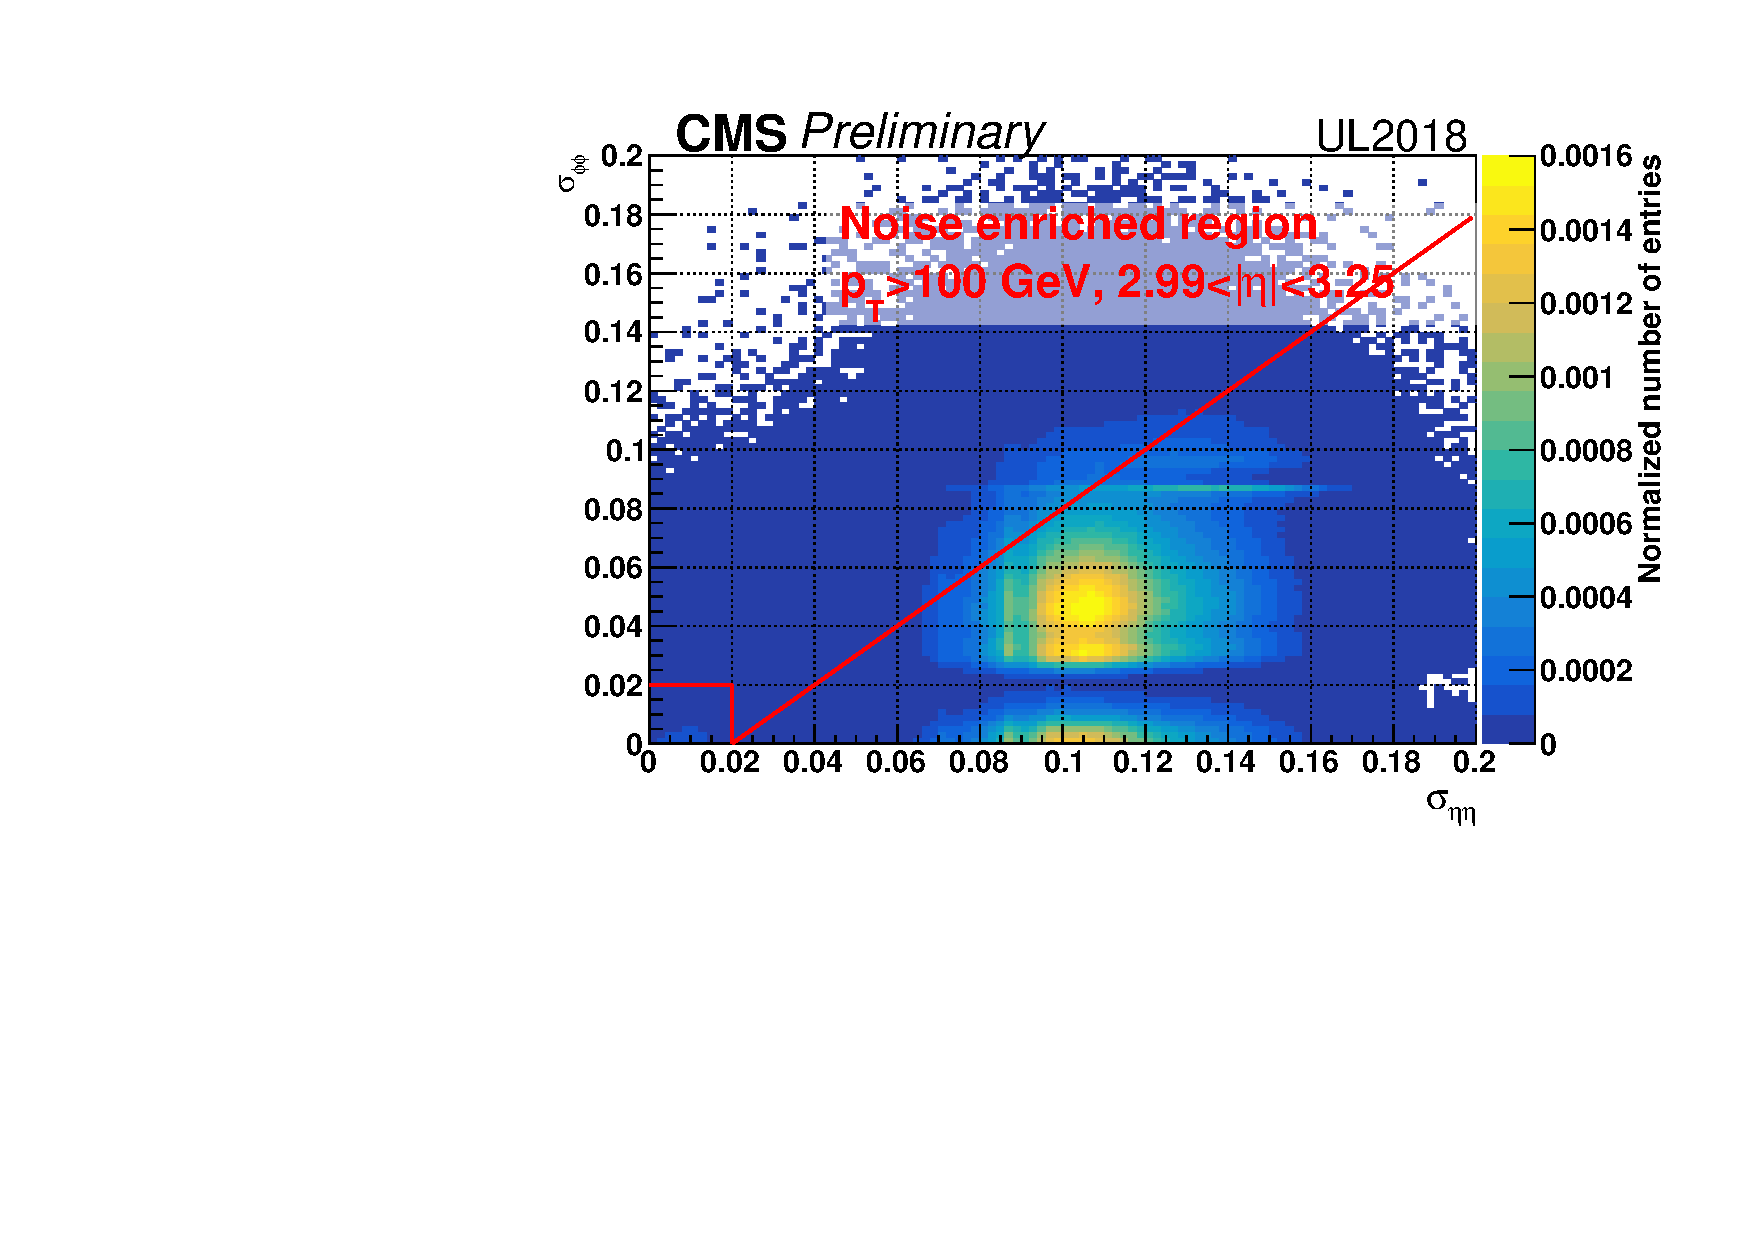
\includegraphics[width=0.45\textwidth]{HFStudy/sigmaetaetavssigmaphiphi_METenriched.pdf}
    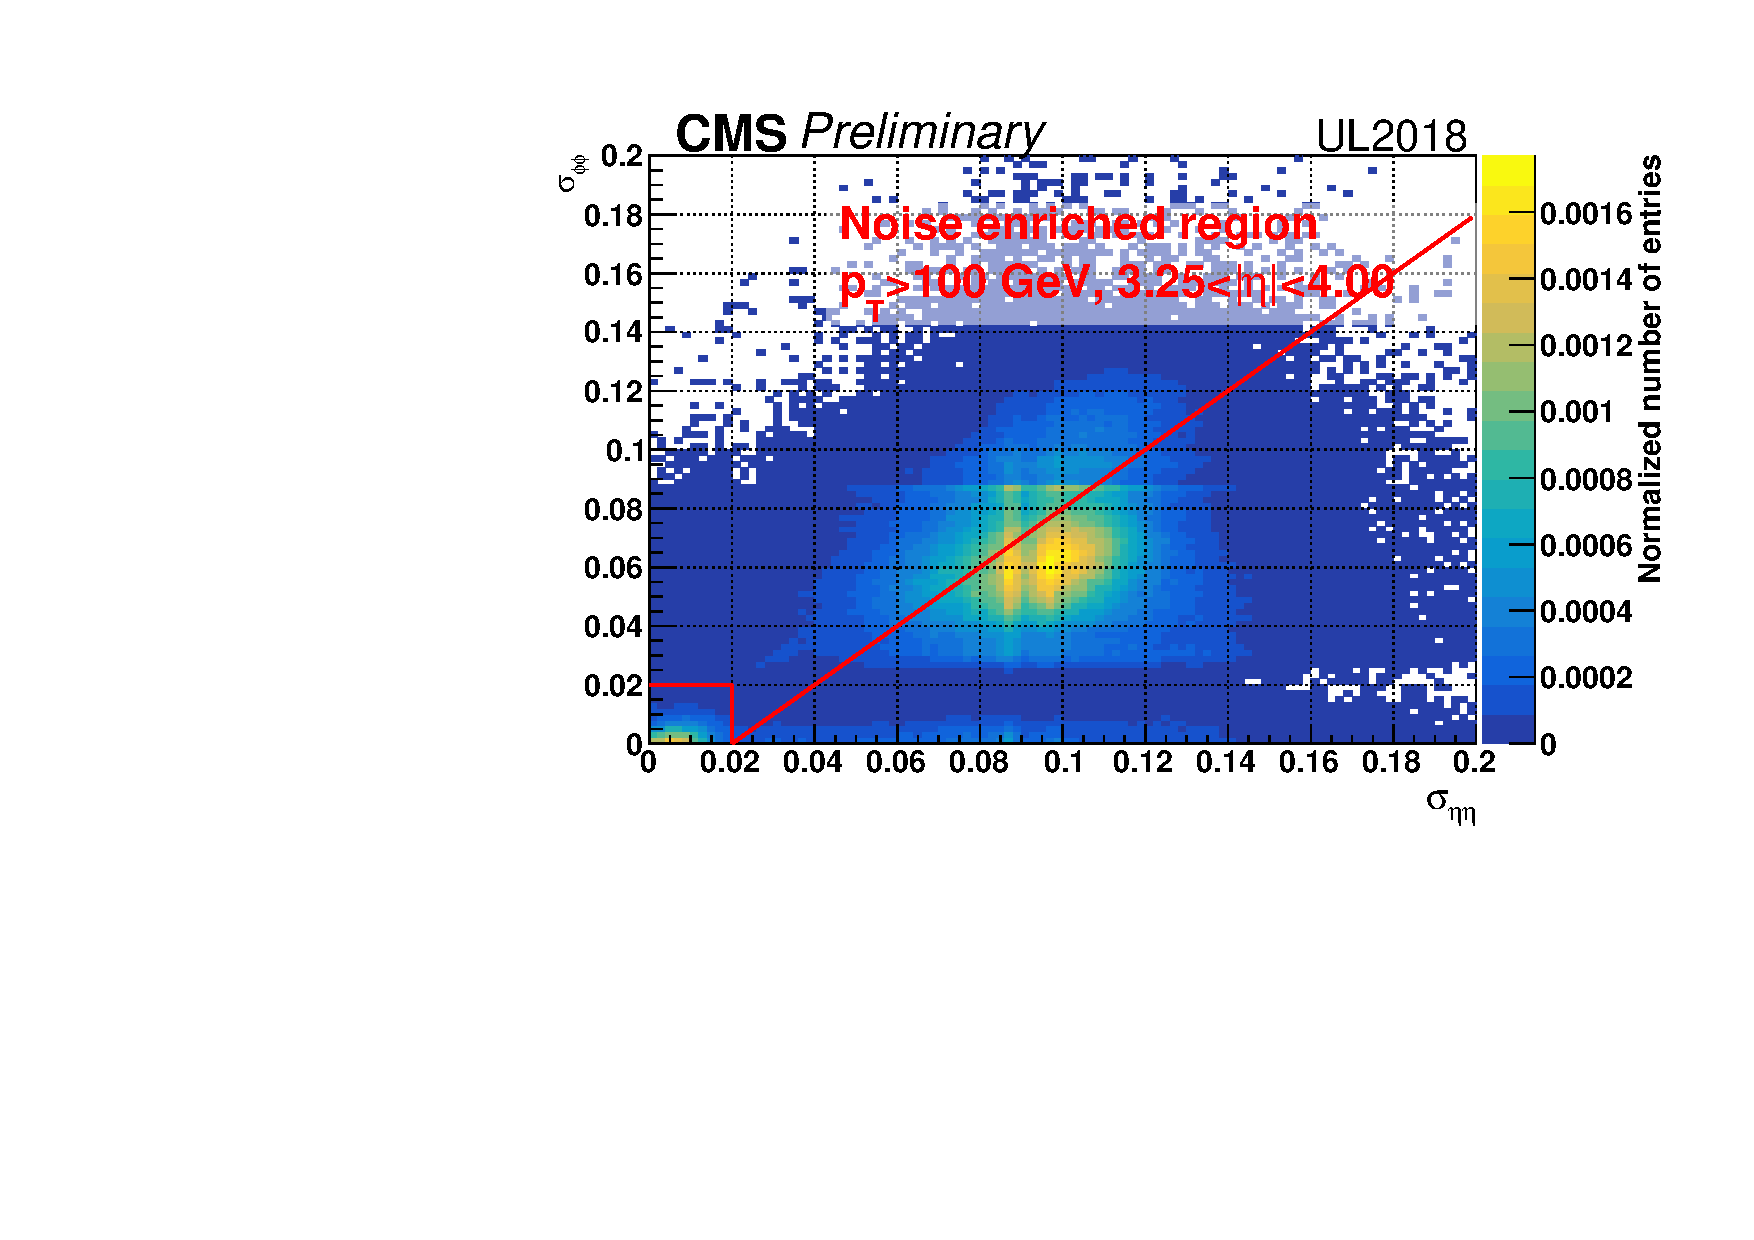
\includegraphics[width=0.45\textwidth]{HFStudy/sigmaetaetavssigmaphiphi_METenriched_eta3p25to4.pdf}
    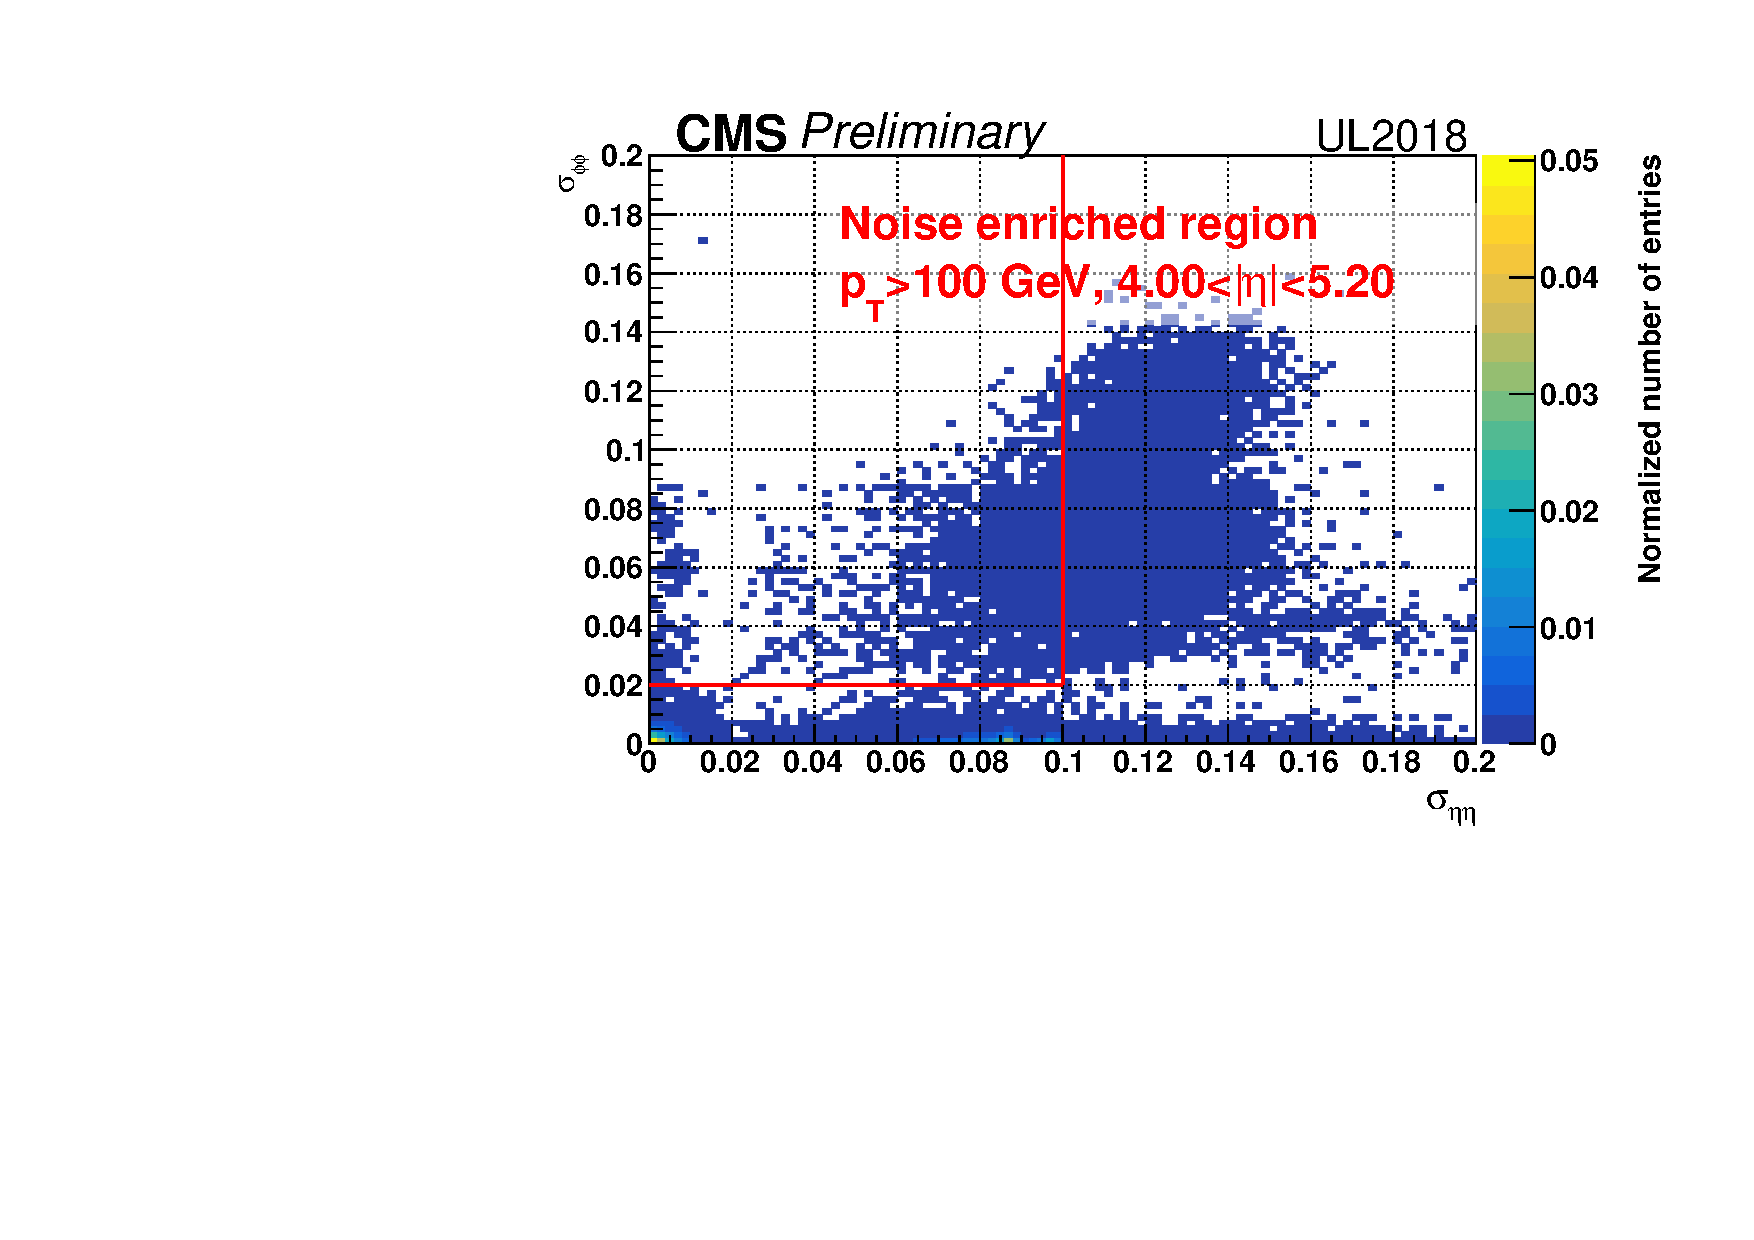
\includegraphics[width=0.45\textwidth]{HFStudy/sigmaetaetavssigmaphiphi_METenriched_eta4to5p2.pdf}
    \caption{Two dimensional distribution of $\sieie$ and $\sipip$ in the noise-enriched region, split by the $|\eta|$ of the jet. The first plot shows 
    $2.99 < |\eta| < 3.25$ interval, the second one shows $3.25 < |\eta| < 4$ and the last one shows $4 < |\eta| < 5.2$. The red lines on the plots indicate
    the cuts applied on these variables.}
    \label{fig:sieie_sipip_noise_enriched}
\end{figure}

\begin{figure}
    \centering
    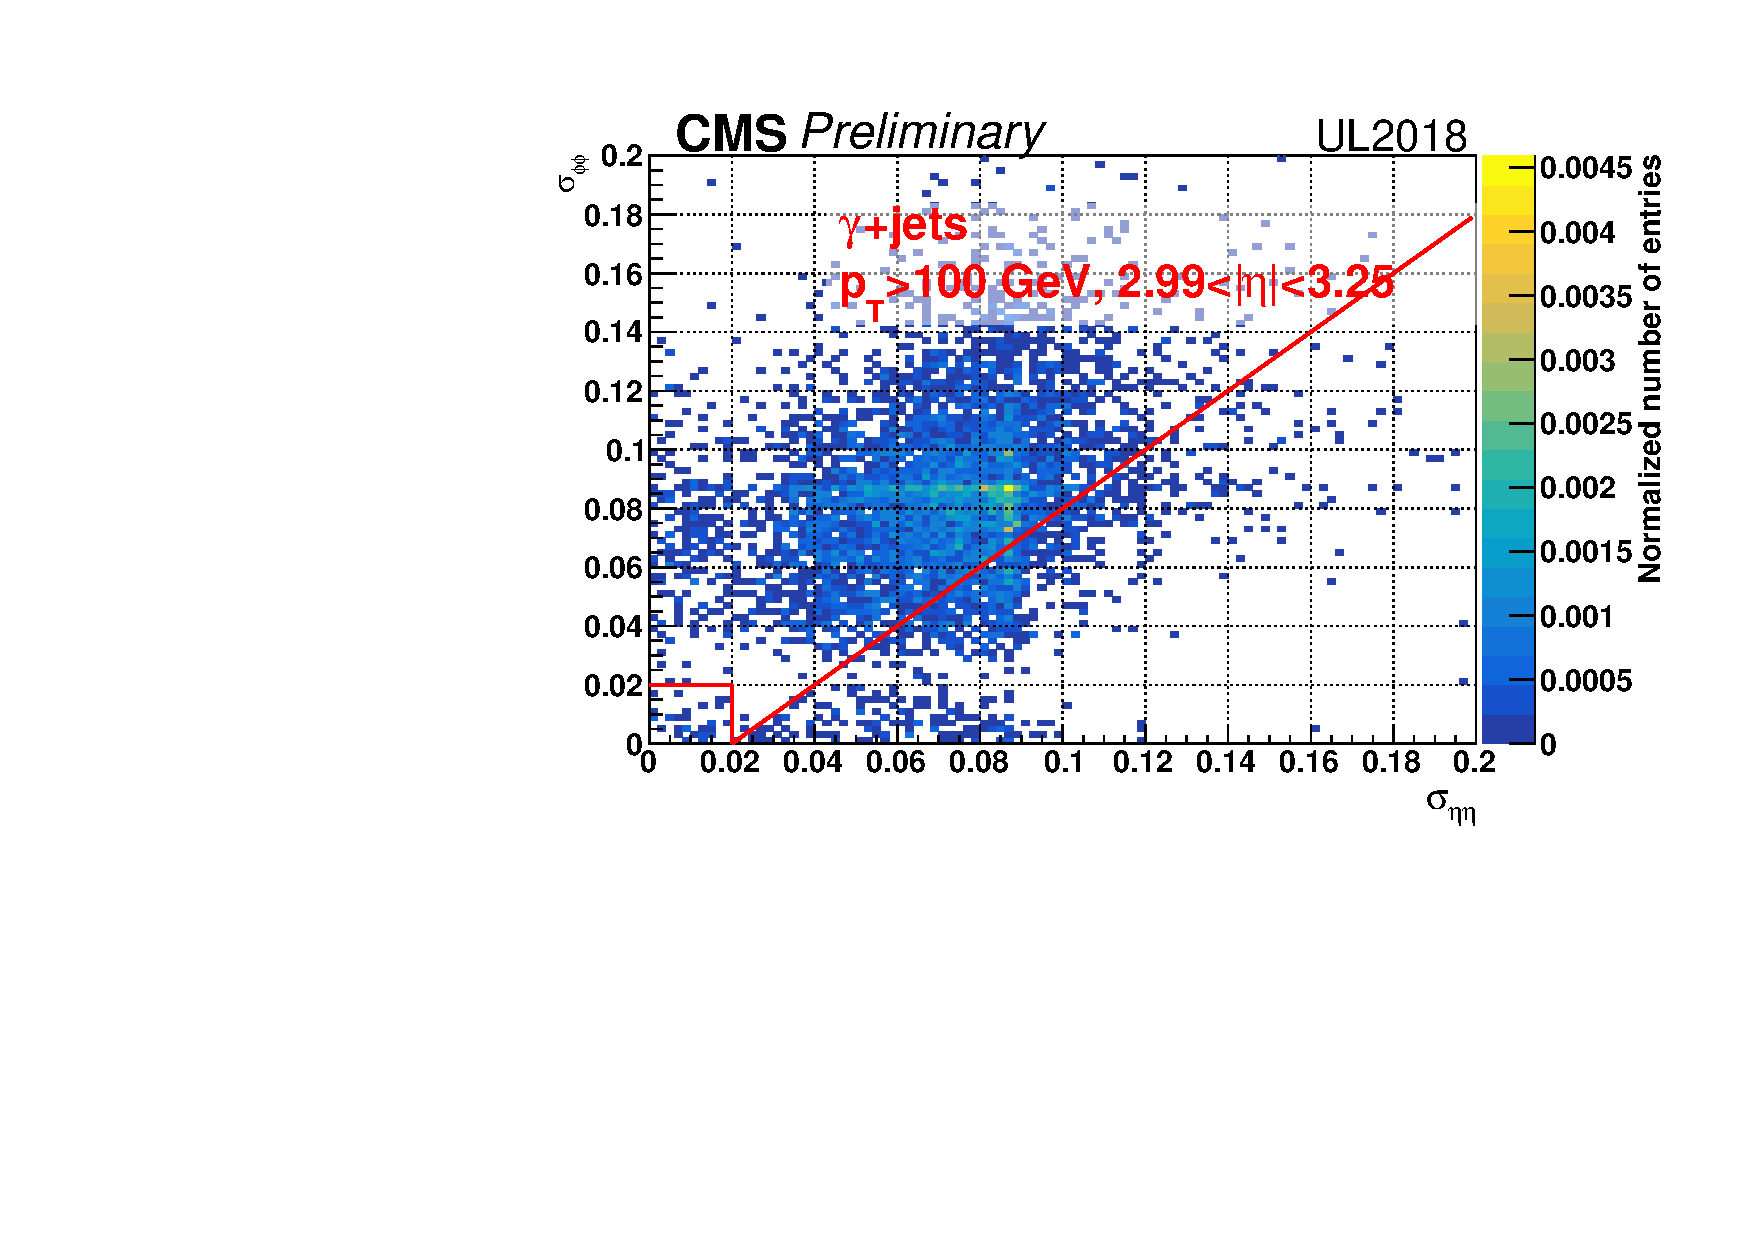
\includegraphics[width=0.45\textwidth]{HFStudy/sigmaetaetavssigmaphiphi_photonjets.pdf}
    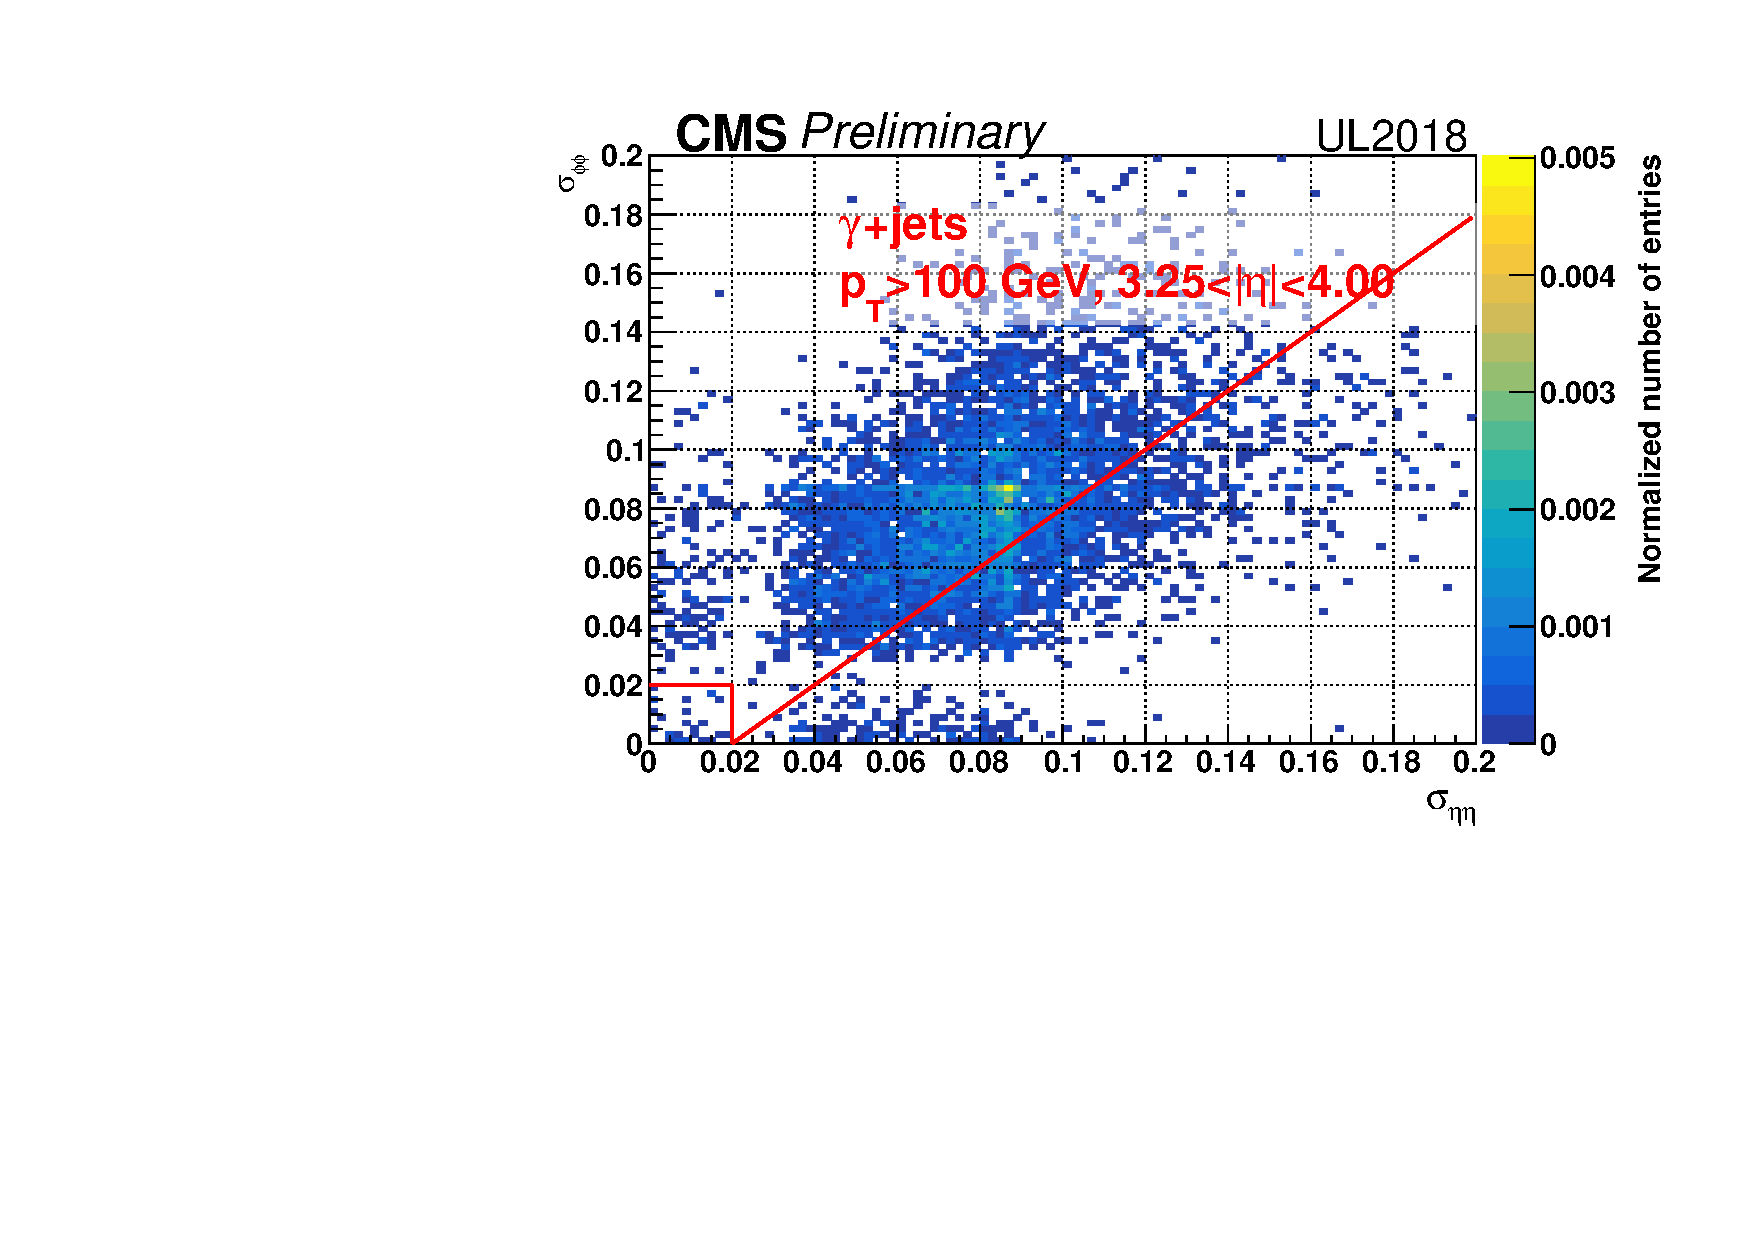
\includegraphics[width=0.45\textwidth]{HFStudy/sigmaetaetavssigmaphiphi_photonjets_eta3p25to4.pdf}
    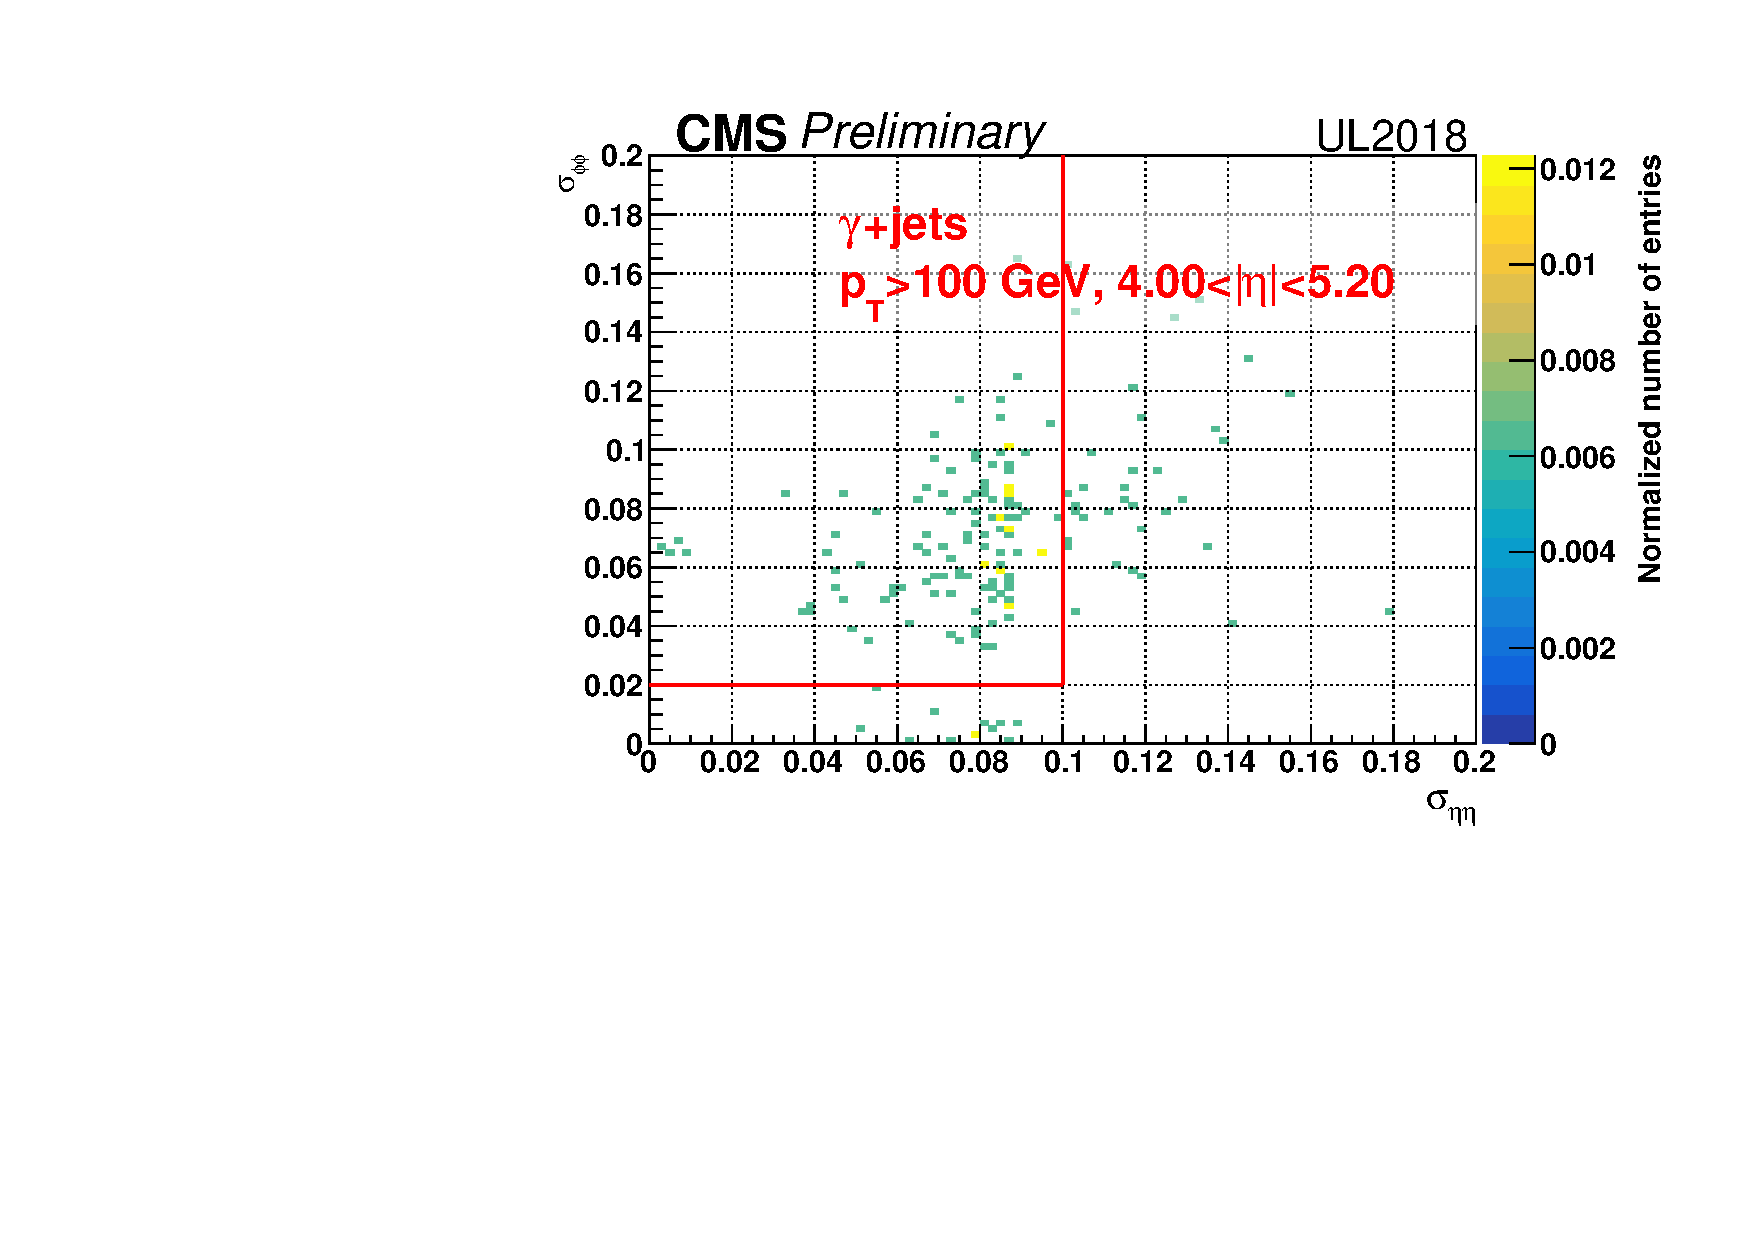
\includegraphics[width=0.45\textwidth]{HFStudy/sigmaetaetavssigmaphiphi_photonjets_eta4to5p2.pdf}
    \caption{Two dimensional distribution of $\sieie$ and $\sipip$ in the physics-enriched region, split by the $|\eta|$ of the jet. The first plot shows 
    $2.99 < |\eta| < 3.25$ interval, the second one shows $3.25 < |\eta| < 4$ and the last one shows $4 < |\eta| < 5.2$. The red lines on the plots indicate
    the cuts applied on these variables.}
    \label{fig:sieie_sipip_physics_enriched}
\end{figure}

The second cut is applied on the HF central strip size ($\hfcss$) of the jet. The two-dimensional distributions of central and adjacent strip sizes for the noise enriched
region are shown in Fig.~\ref{fig:stripsize_noise_enriched}, while the same distributions in the physics enriched region are shown in Fig.~\ref{fig:stripsize_phys_enriched}.
For the jets in noise enriched region with $2.99 < |\eta| < 3.25$ (where the noise contribution is the highest), it can be observed that around $40\%$ of jets
have $\hfcss \geq 3$, while in the physics enriched region, this fraction is very small, $\mathcal{O}(1\%)$. Therefore, a cut on the $\hfcss$ variable is adopted in 
the analysis, requiring $\hfcss < 3$ for HF jets that are back to back with $\ptmiss$. 

\begin{figure}
    \centering
    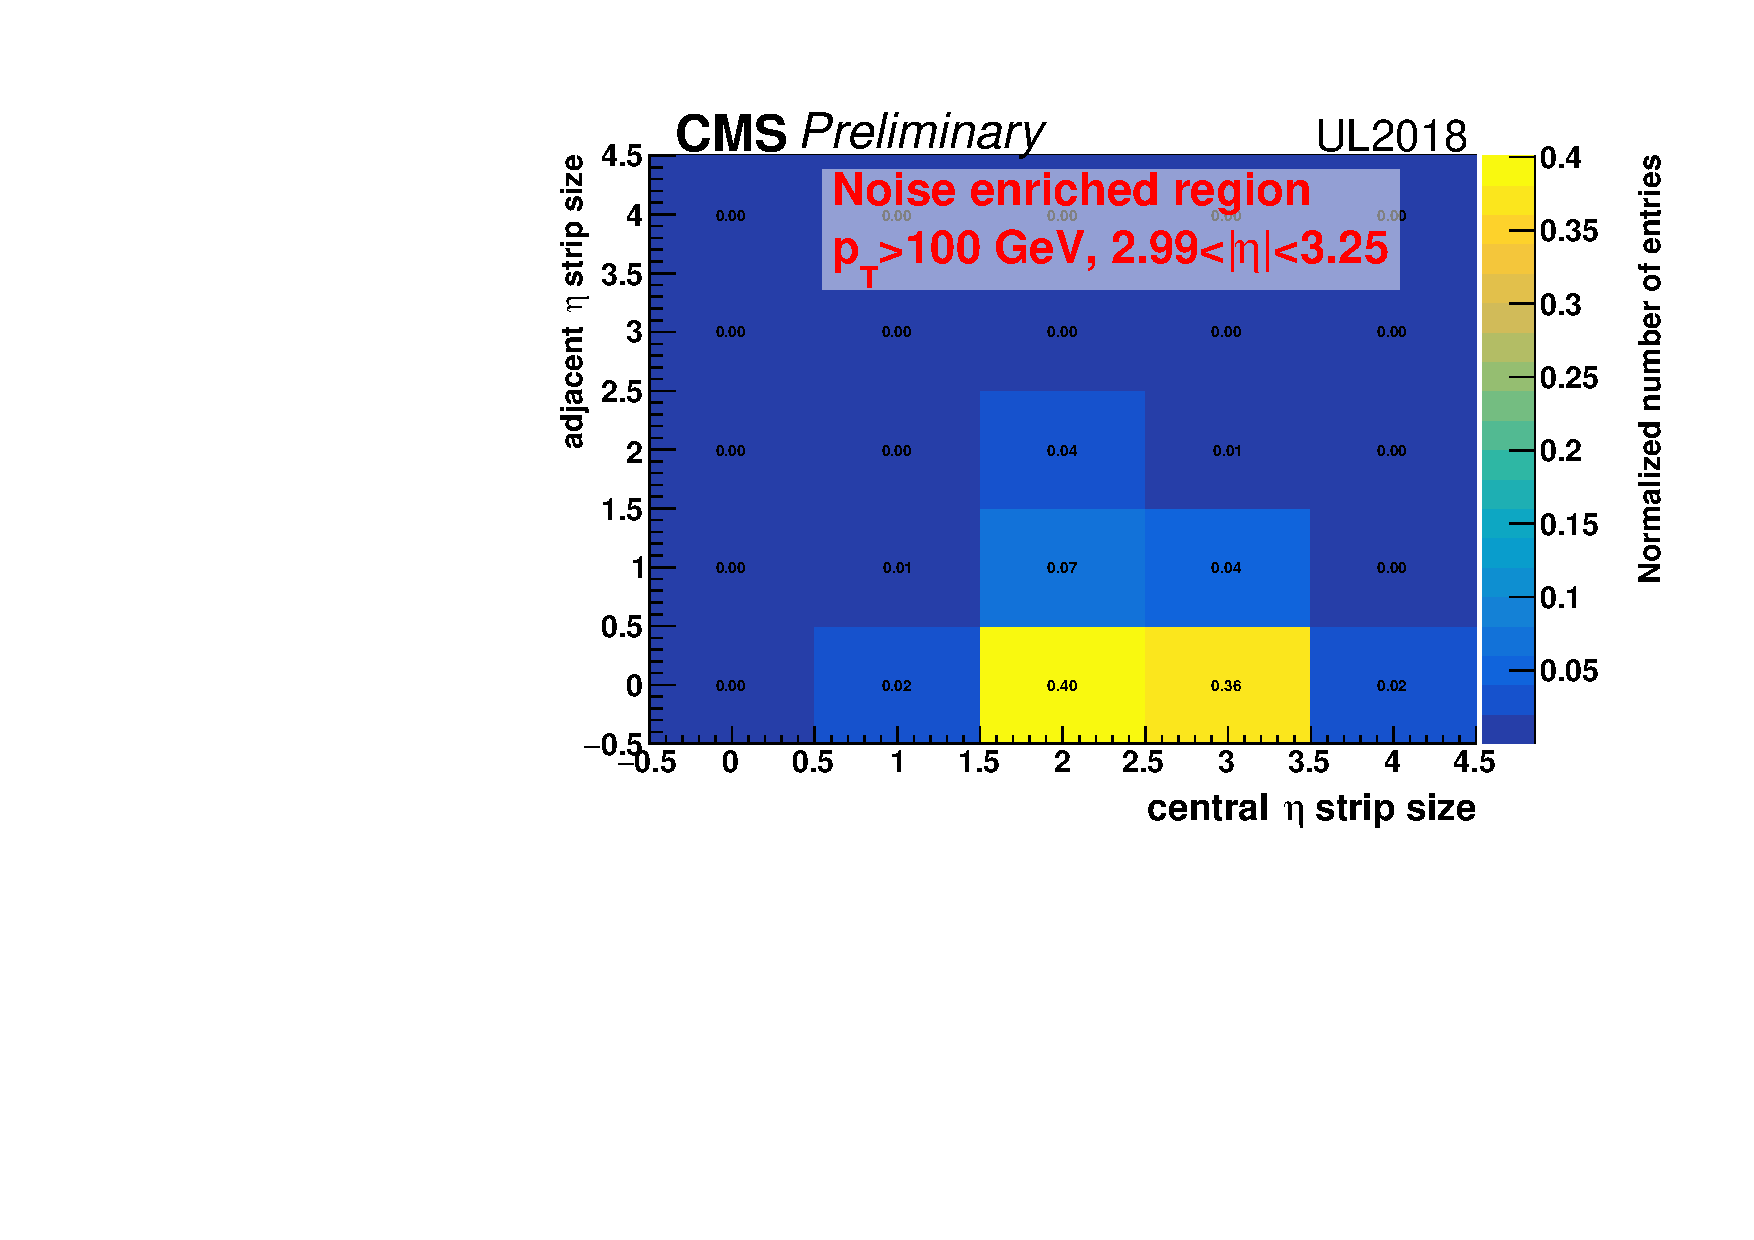
\includegraphics[width=0.45\textwidth]{HFStudy/etasizecentralvsadj_METenriched.pdf}
    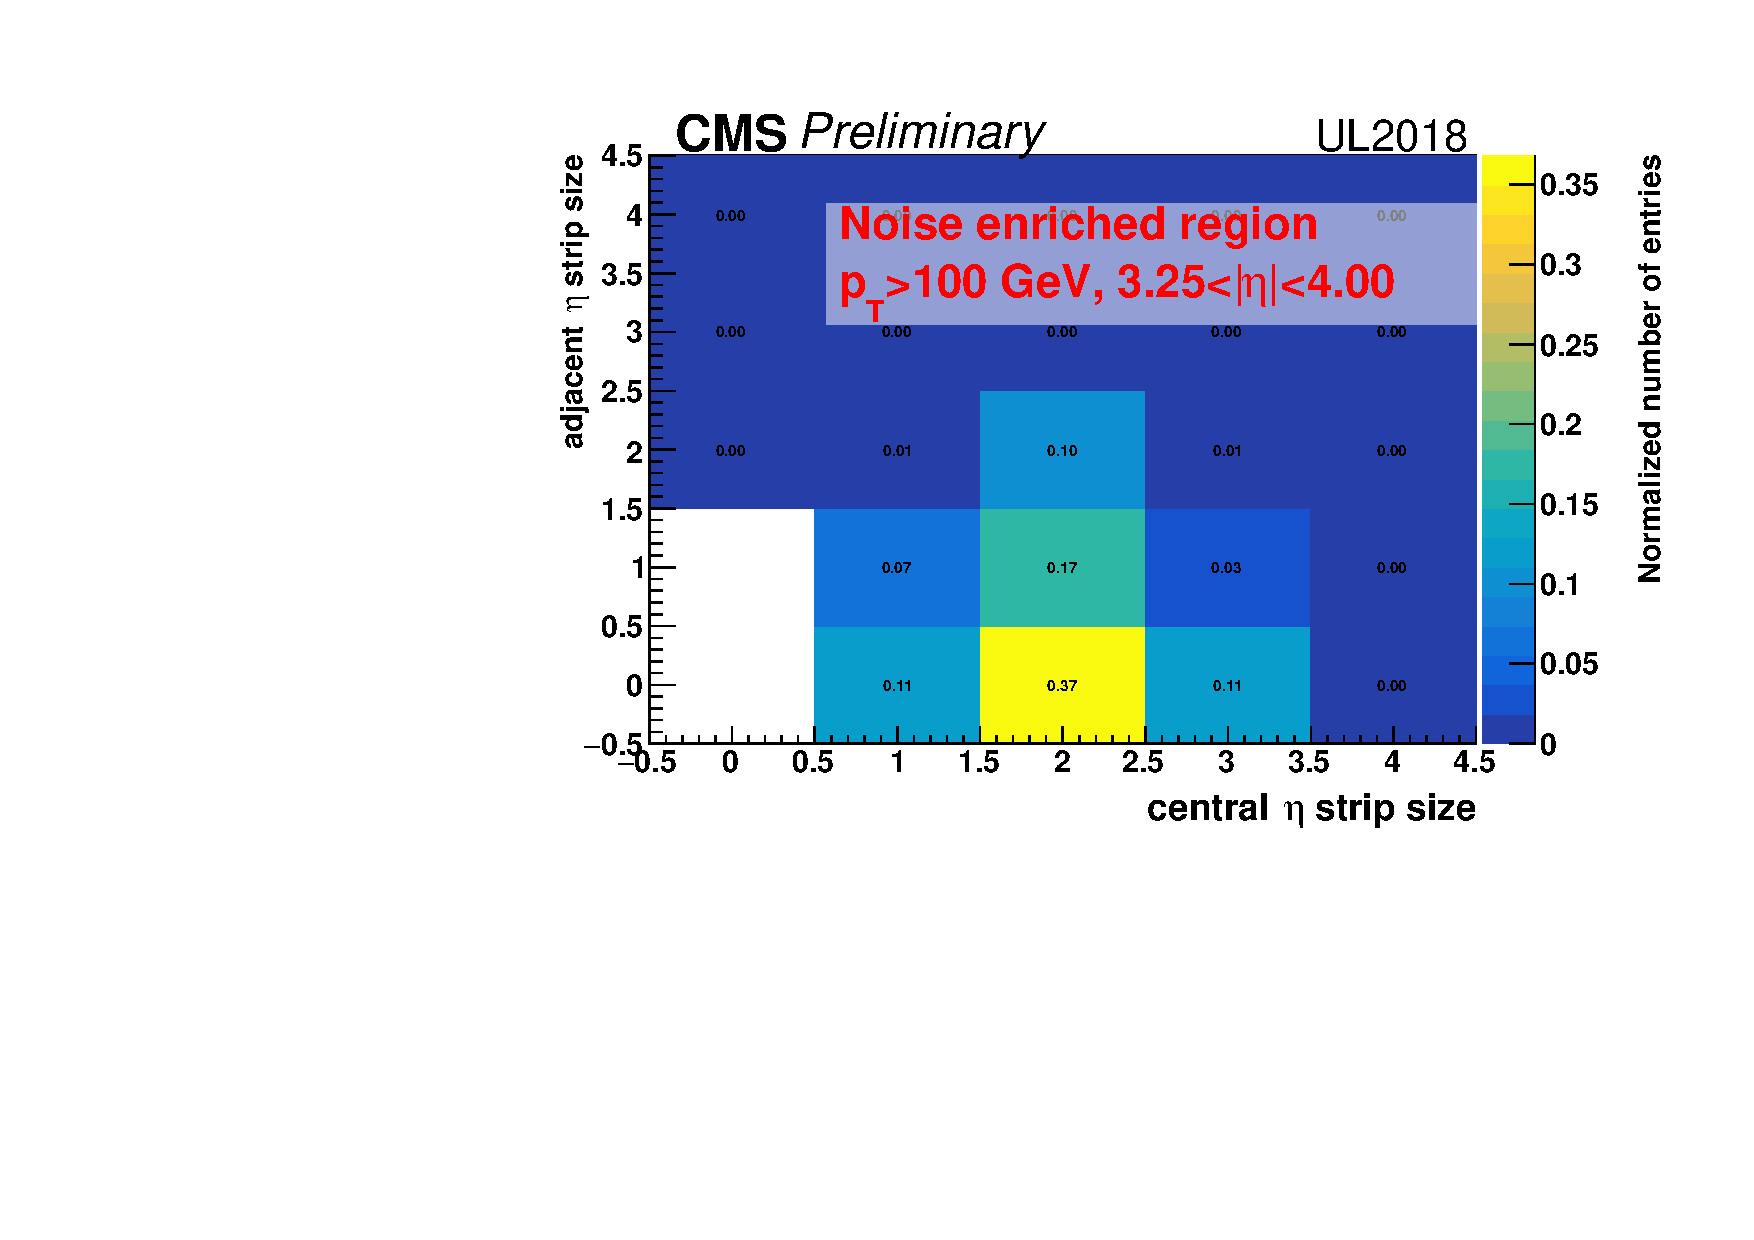
\includegraphics[width=0.45\textwidth]{HFStudy/etasizecentralvsadj_METenriched_eta3p25to4.pdf}
    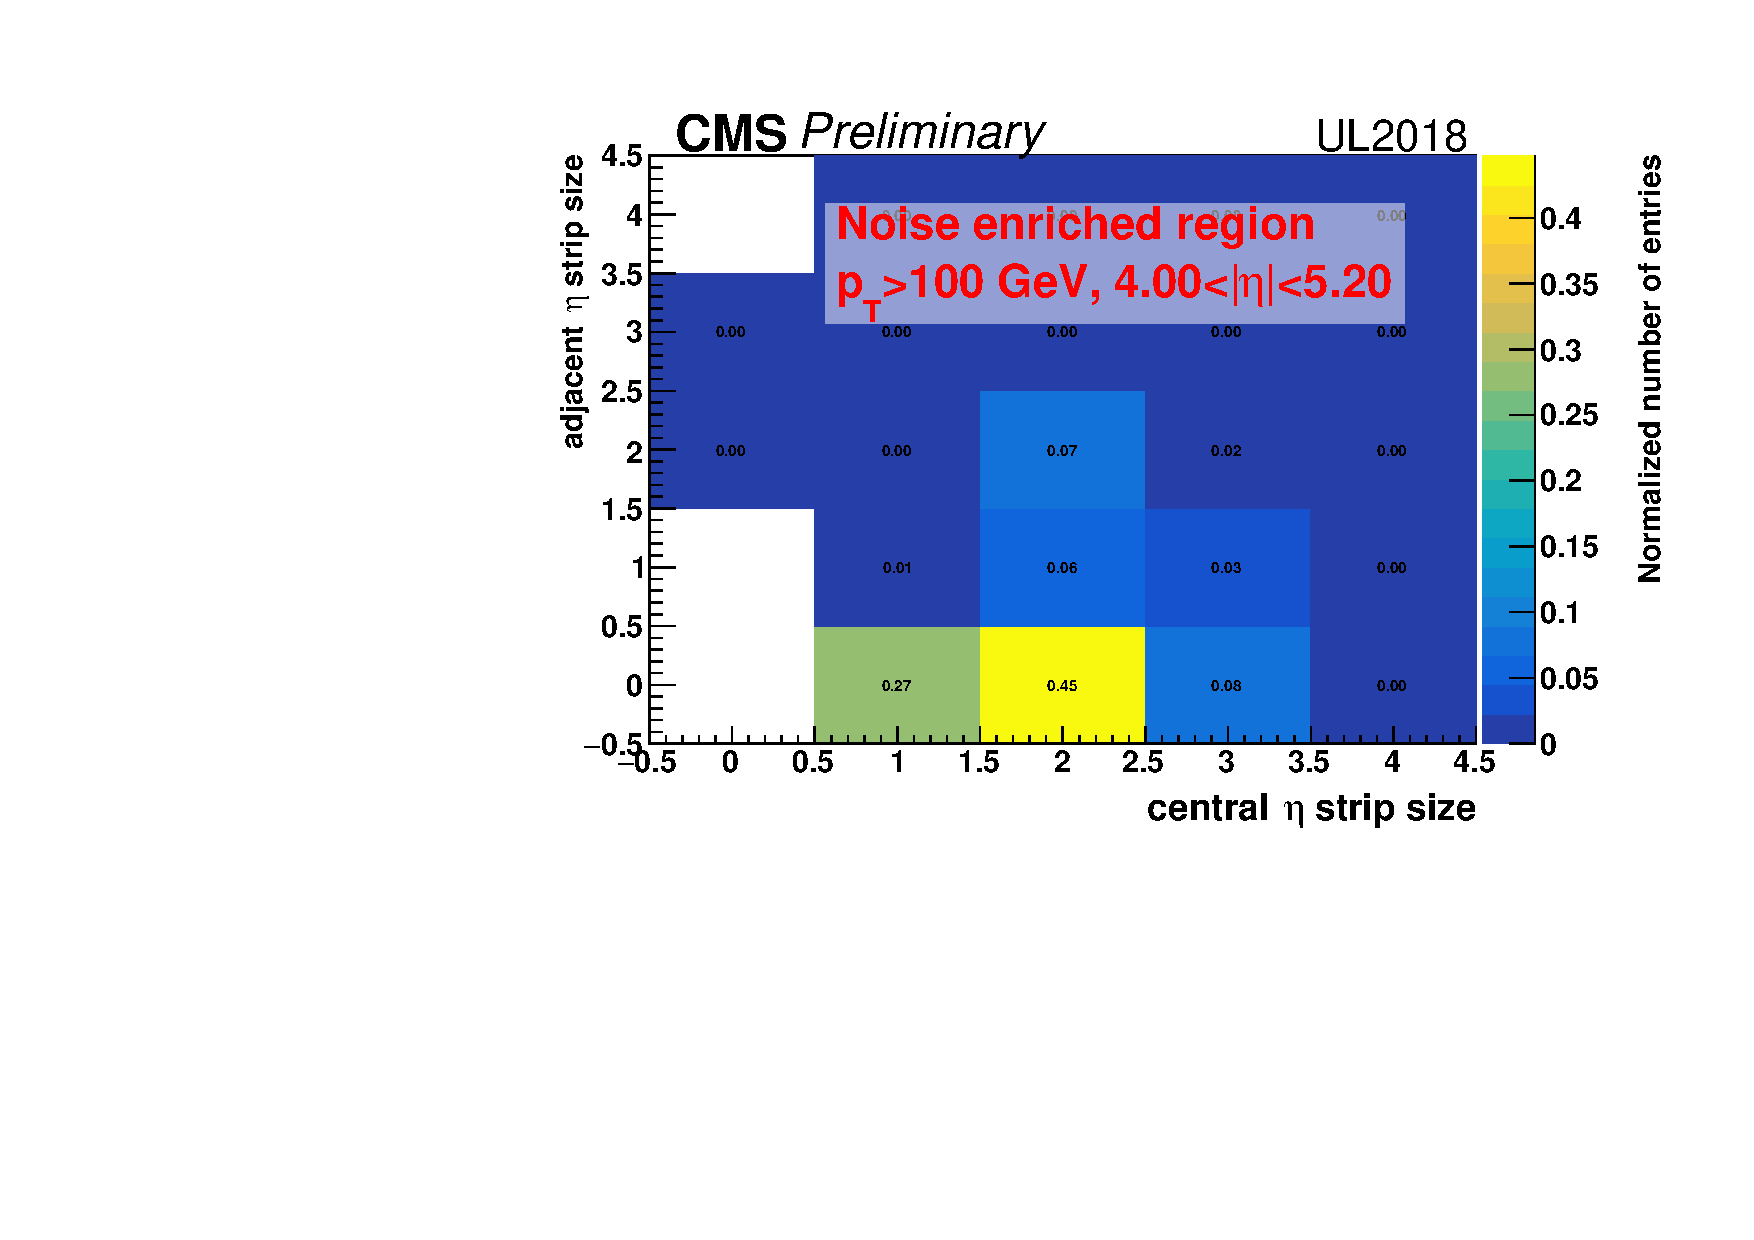
\includegraphics[width=0.45\textwidth]{HFStudy/etasizecentralvsadj_METenriched_eta4to5p2.pdf}
    \caption{Two dimensional distribution of central and adjacent strip sizes in the noise enriched region, split by the $|\eta|$ of the jet. The first plot shows 
    $2.99 < |\eta| < 3.25$ interval, the second one shows $3.25 < |\eta| < 4$ and the last one shows $4 < |\eta| < 5.2$.}
    \label{fig:stripsize_noise_enriched}
\end{figure}

\begin{figure}
    \centering
    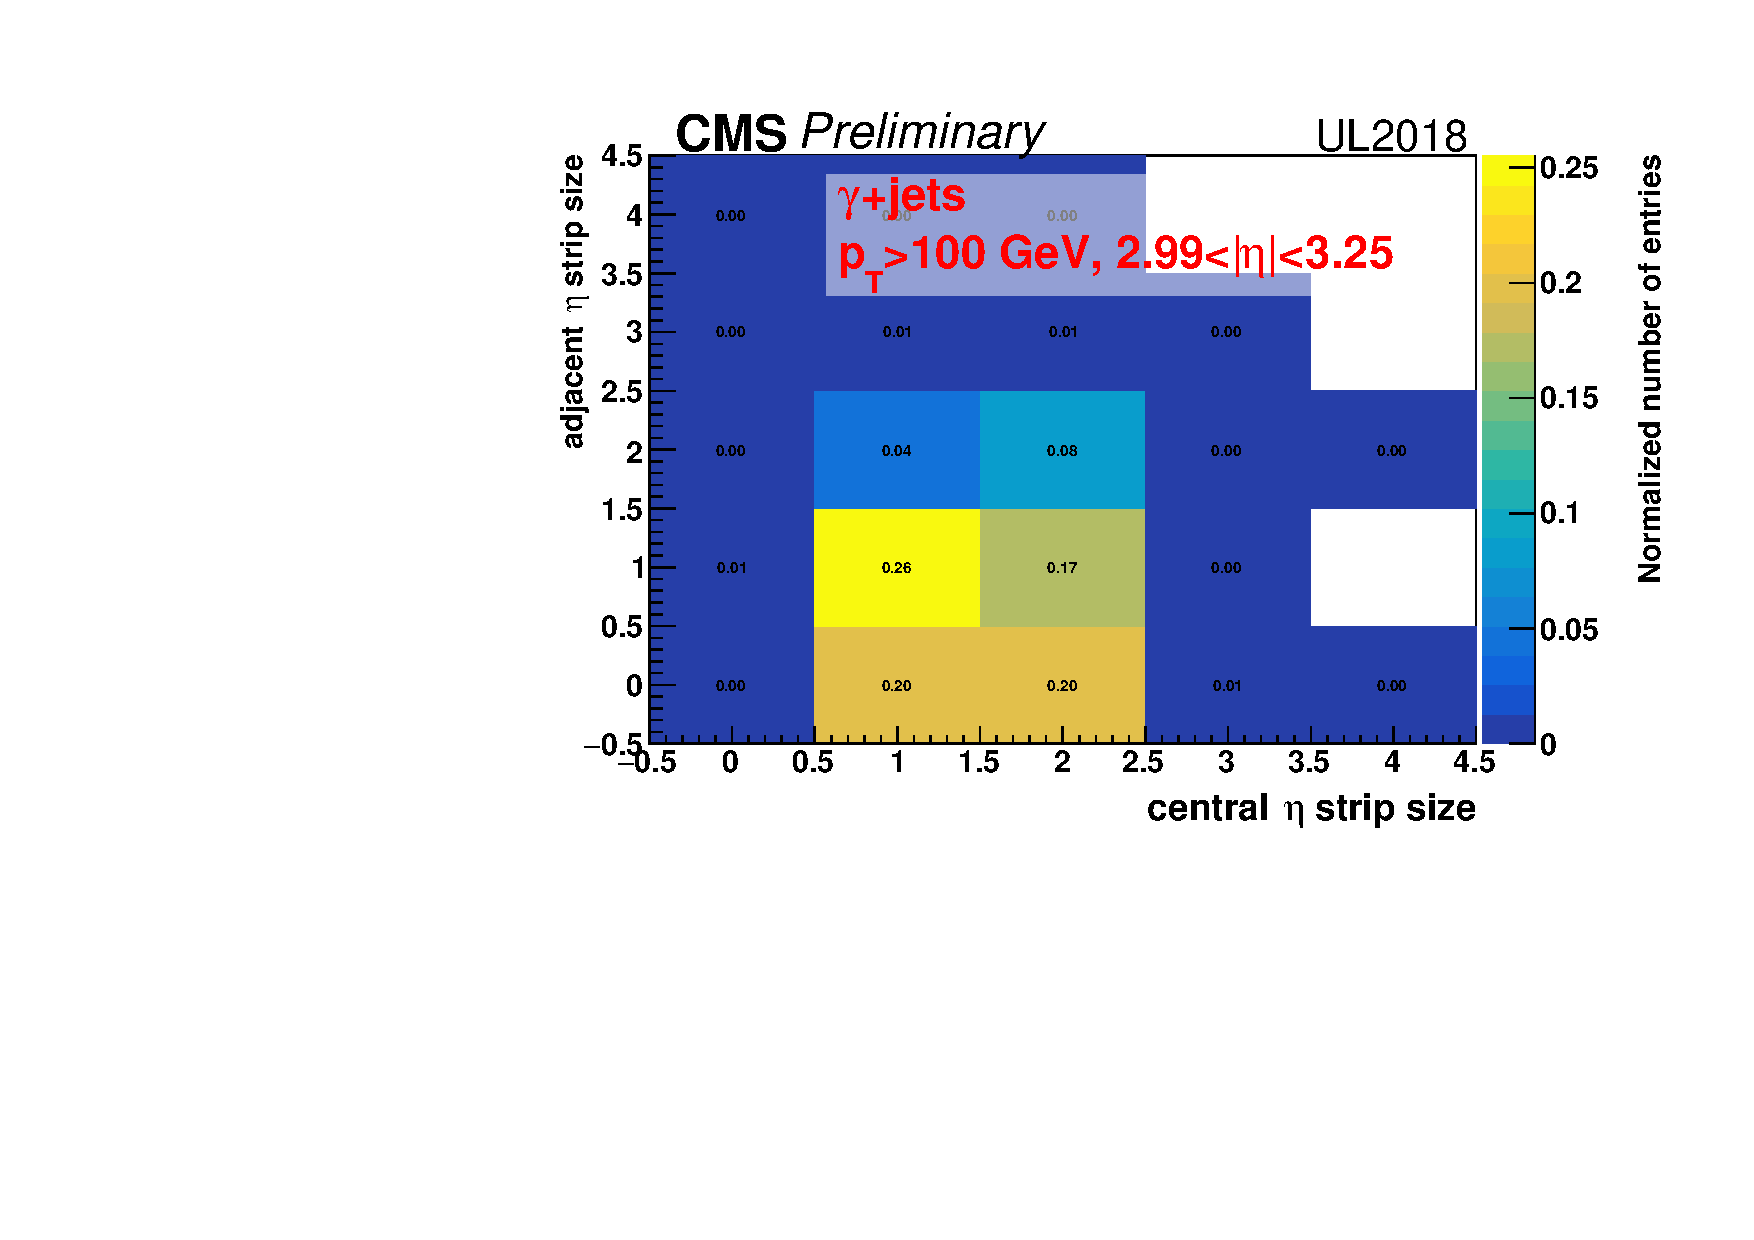
\includegraphics[width=0.45\textwidth]{HFStudy/etasizecentralvsadj_gammajets.pdf}
    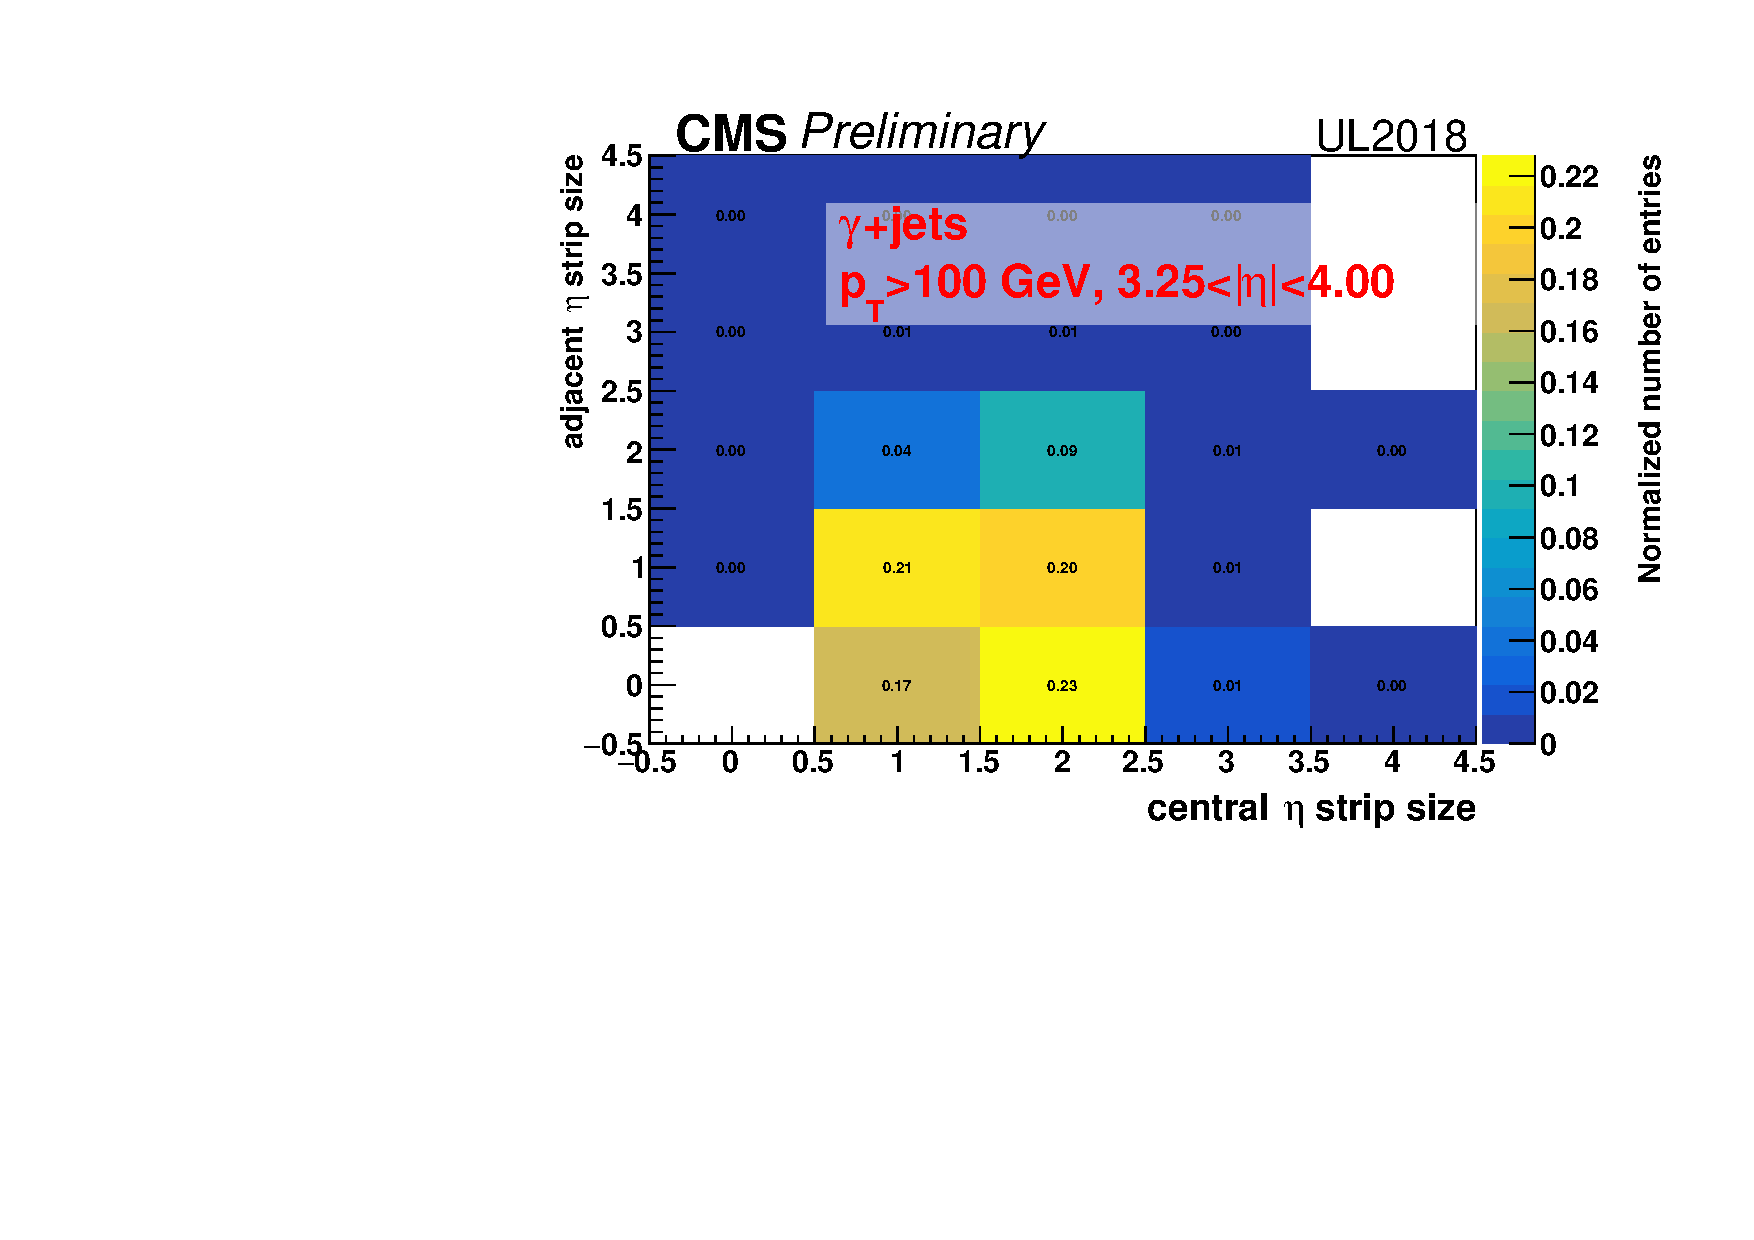
\includegraphics[width=0.45\textwidth]{HFStudy/etasizecentralvsadj_gammajets_eta3p25to4.pdf}
    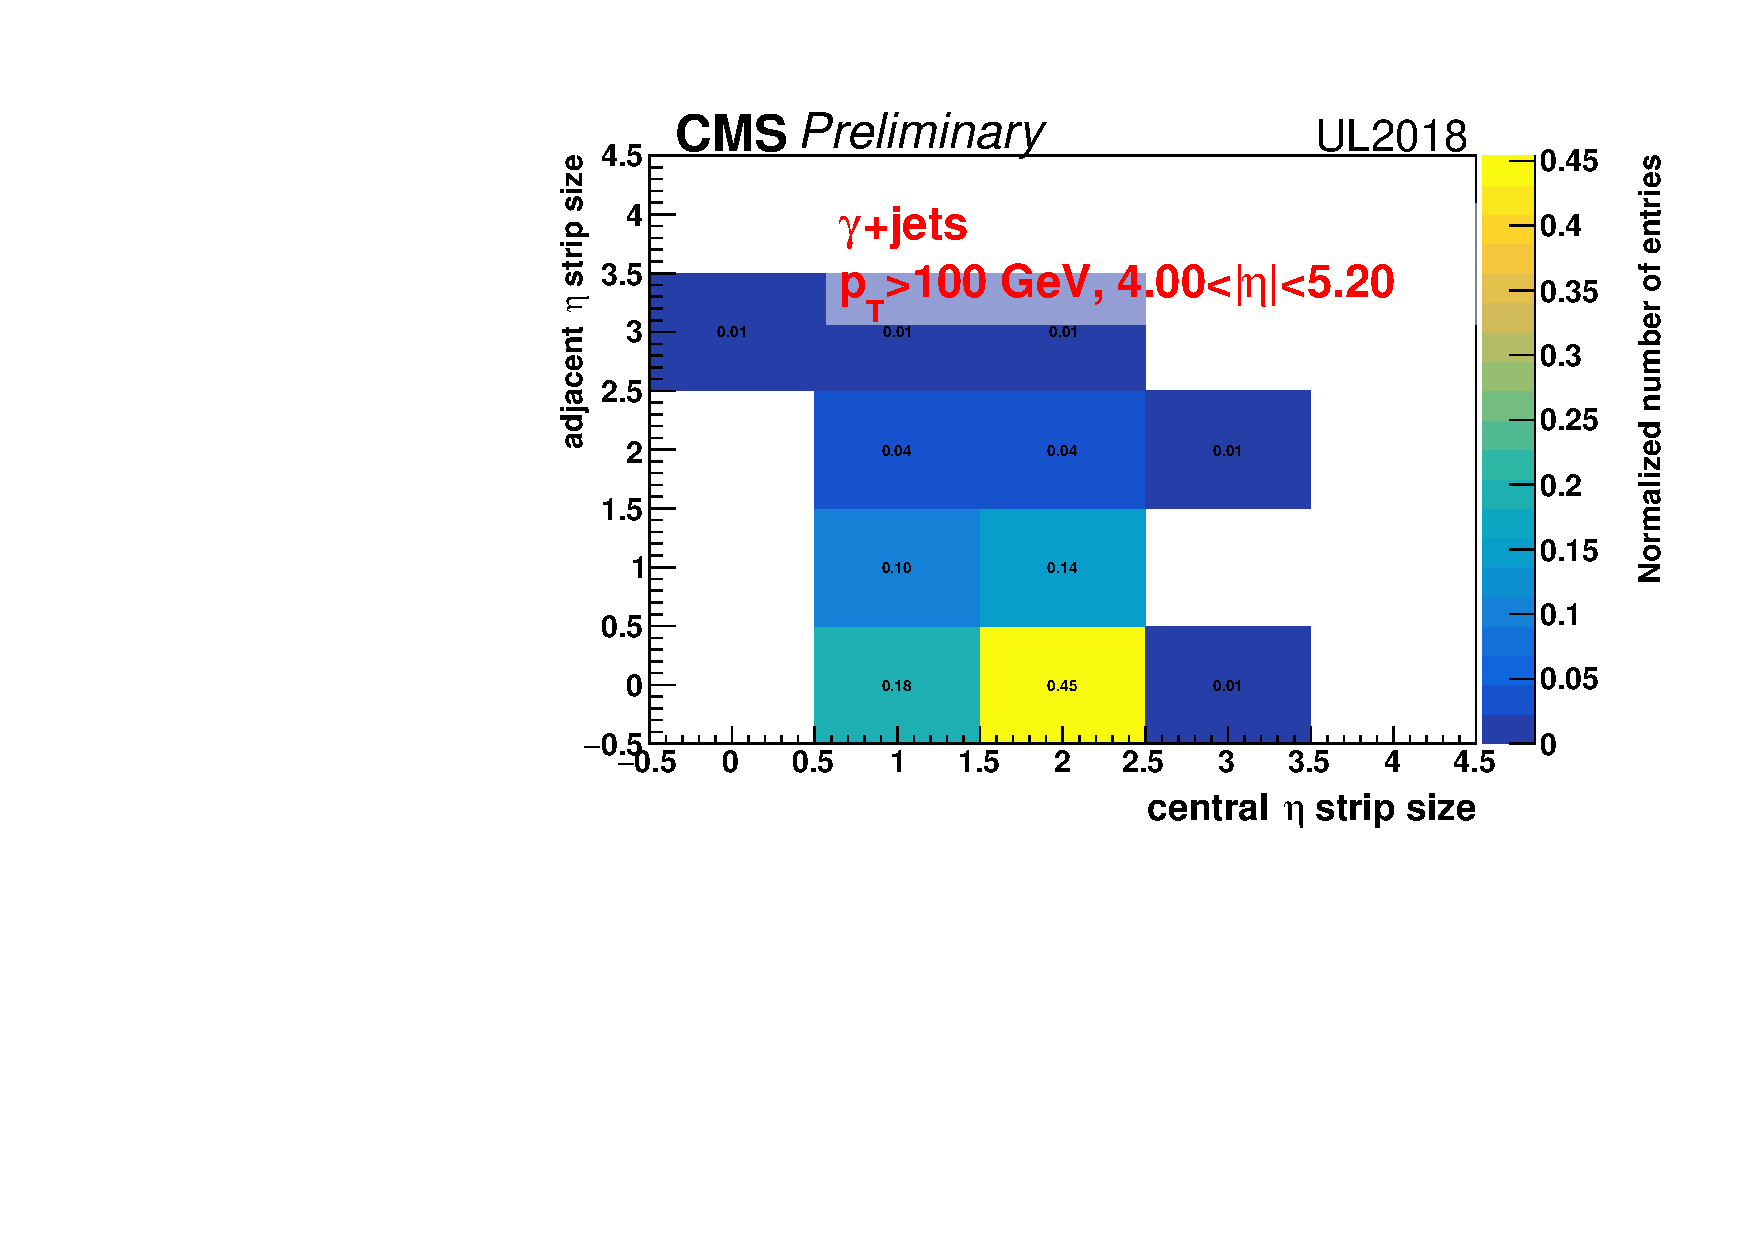
\includegraphics[width=0.45\textwidth]{HFStudy/etasizecentralvsadj_gammajets_eta4to5p2.pdf}
    \caption{Two dimensional distribution of central and adjacent strip sizes in the physics enriched region, split by the $|\eta|$ of the jet. The first plot shows 
    $2.99 < |\eta| < 3.25$ interval, the second one shows $3.25 < |\eta| < 4$ and the last one shows $4 < |\eta| < 5.2$.}
    \label{fig:stripsize_phys_enriched}
\end{figure}


In summary, the cleaning cuts applied to HF jets are:
\begin{itemize}
    \item $2.99 < |\eta| < 4.0$: $\sieie - \sipip < 0.02$ condition is required. In addition, the corner region, defined as $\sieie < 0.02 \ \& \ \sipip < 0.02$,
    is also removed from the analysis.
    \item $|\eta| > 4.0$: $\sieie < 0.1 \ \& \ \sipip > 0.2$ condition is required.
    \item $|\eta| > 2.99$: $\hfcss < 3$ is required.
\end{itemize}

They are applied to all jets with $\pt > 100$ GeV and $|\eta| > 2.99$ that are back-to-back with $\ptmiss$
(i.e. $\Delta\phi(jet,\ptmiss) > 2.5$). If any such jet fails the cuts, the event is rejected. 


\subsubsection{Residual HF Noise Estimation}
\label{subsubsec:hf_noise_est}

In addition to the HF cleaning cuts explained in the previous subsection,
a noise estimation is done to estimate the leftover noise contribution in  
the analysis signal region. For the noise estimation, a new control region is defined
in which the HF shape cuts are inverted. Other than the HF shape cuts,
the same cuts are required in this control region as in the VBF signal region, which are
discussed in Sec.~\ref{subsec:sr_vbf_selection}. For the remainder of this text, this control
region will be referred to as HF control region.

With the addition of this HF control region (CR), the estimation is done in three steps.
First, data and MC yields in this CR are computed ($N_{data}$, $N_{MC}$). The excess amount of data over MC 
in this control region gives the number of excess events in data with HF noise, not modeled by the 
simulation: $N_{noise}^{CR} = N_{data} - N_{MC}$. 
Finally, the noise estimate in analysis signal region is calculated from $N_{noise}^{CR}$ by using $[\pt, \eta]$ dependent transfer factors,
defined as the relative probability for a noise event to pass the HF shape cuts, relative to failing them.
This probability is derived from events in a noise-enriched region, where the probability of a jet in such an event
to pass the HF cuts can be computed as a function of its pseudorapidity and transverse momentum, $\hfprobpass[p_{T}, \eta]$.
Using these probabilities, the transfer factor $R_{jet}$ for a single jet can be then written as:

\begin{equation}
    R_{jet} (p_T, \eta) = \frac{\hfprobpass}{\hfprobfail} (p_T, \eta) = \frac{\hfprobpass}{1 - \hfprobpass} (p_T, \eta)
\end{equation}

For a given event, the total transfer factor (taking all HF jets into account in the event) can be then computed as

\begin{equation}
    R_{event} = \prod_{jet} R_{jet} (p_T, \eta)
\end{equation}

where the product runs over the jets in the event with $p_T > 100$ GeV and $|eta| > 2.99$ (i.e. HF jets). If there are no
jets in the event that satisfy this criteria, $R_{event}$ is defined to be $0$, signifying the fact that there will be no contribution
to the signal region noise estimate template from this event. If there is such a jet however, $R_{event} \neq 0$, hence signifying
a non-zero contribution to the noise estimation in the signal region.

In this way, the contribution of a single event in the noise-enriched CR to the HF noise template in the signal region can be written as

\begin{equation}
    N_{noise}^{SR} = R_{event} \times (N_{data}^{CR} - N_{MC}^{CR})
    \label{eq:hf_noise_calc_single_event}
\end{equation}

Eq.~\ref{eq:hf_noise_calc_single_event} shows the contribution from a single event in the HF control region.
As the final step, summing up the contributions from all events in the HF control region gives the full $\mjj$ 
noise estimate template for the HF noise, which are shown in Fig.~\ref{fig:hf_estimation_mtr}.
Plots on the left column show the data and total MC
yields in the HF control region, each event being already scaled by the transfer factor 
$R_{event}$ as defined above. 
Plots on the right column show the resulting HF noise estimation in the analysis
signal region, which correspond to the difference of data and MC yields in the left-hand side plots.
Plots on the top show the results with 2017 data, and plots on the bottom show results with 2018 data.

\begin{figure}[h!]
    \centering
        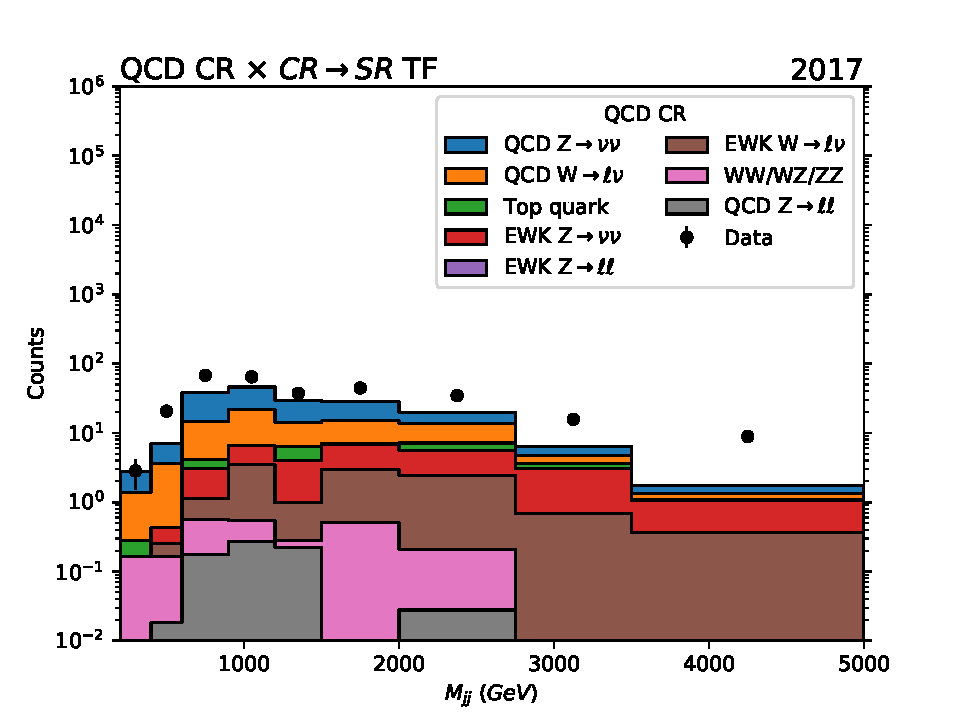
\includegraphics[width=0.49\textwidth]{HFStudy/NoiseEstimation/cr_vbf_qcd_mjj_2017.pdf}
        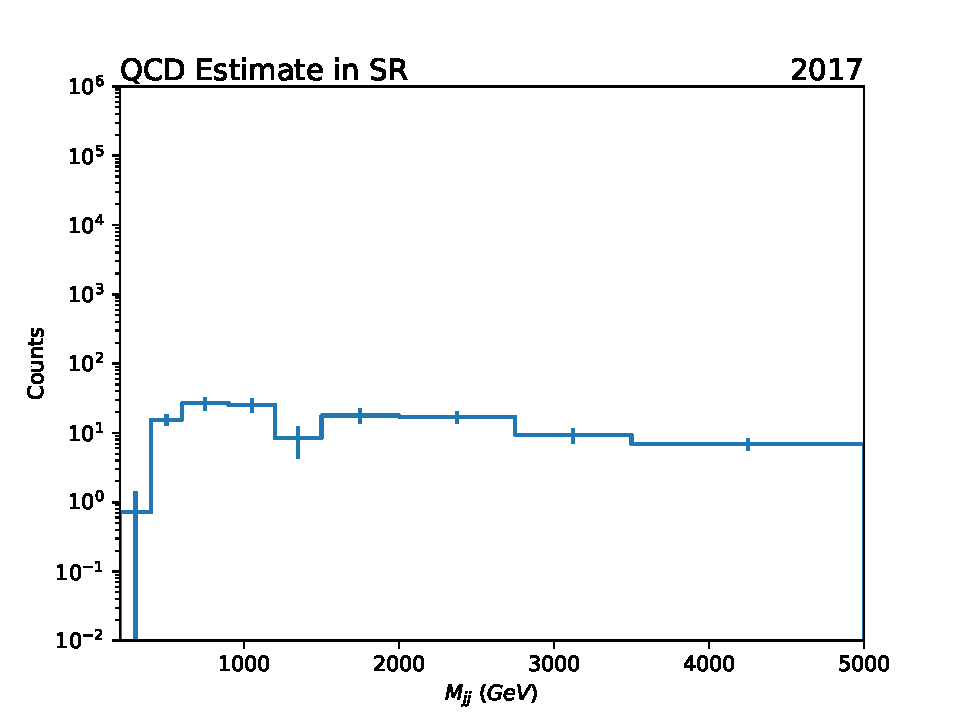
\includegraphics[width=0.49\textwidth]{HFStudy/NoiseEstimation/qcd_estimation_mjj_2017.pdf} \\ 
        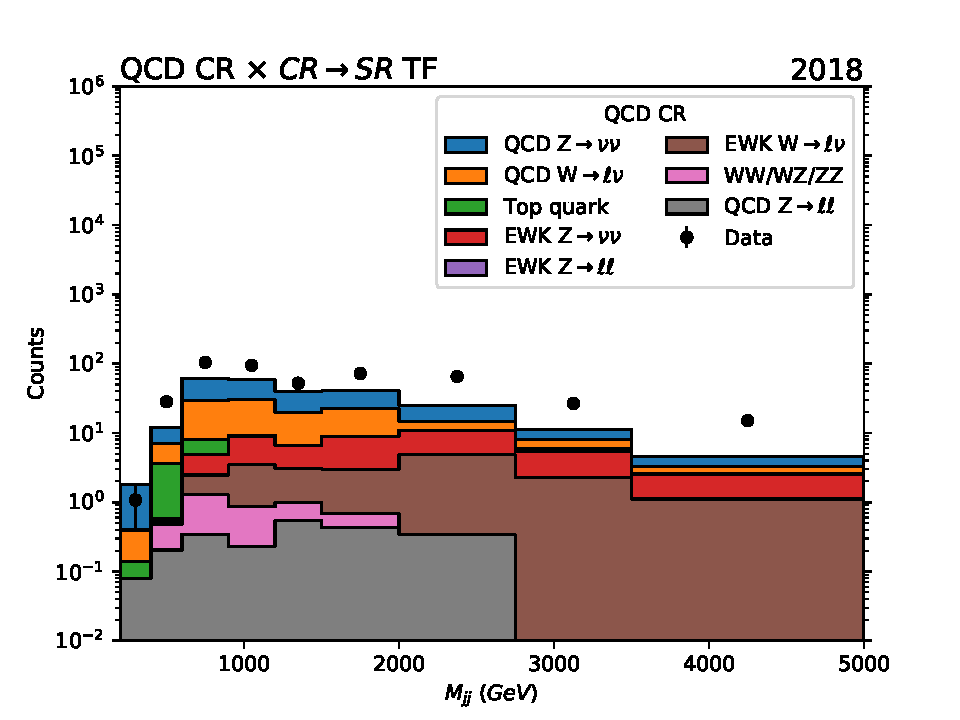
\includegraphics[width=0.49\textwidth]{HFStudy/NoiseEstimation/cr_vbf_qcd_mjj_2018.pdf}
        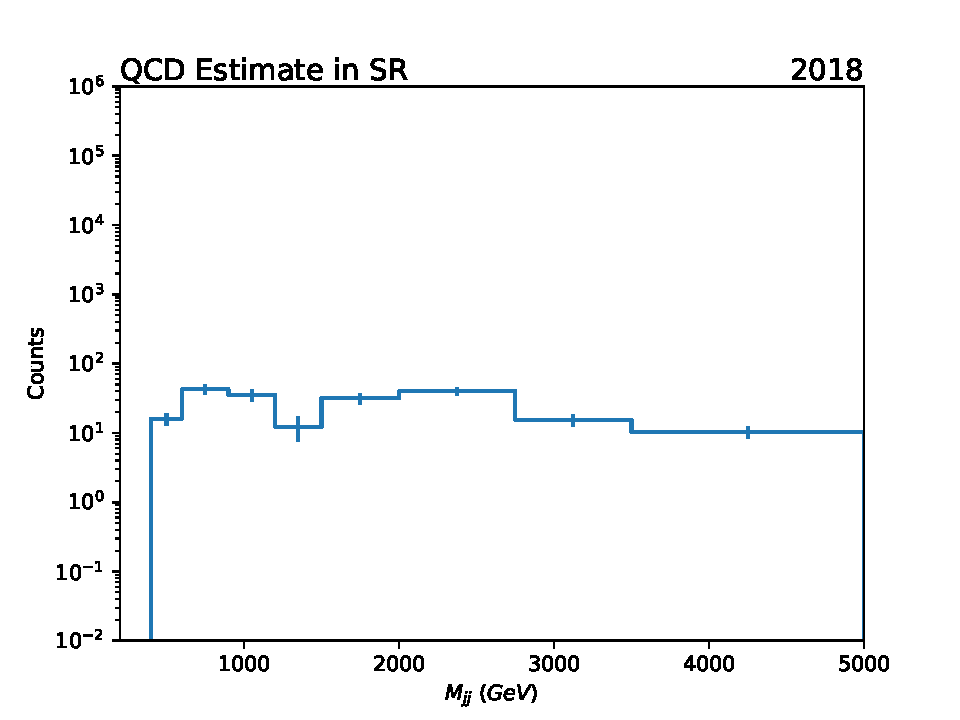
\includegraphics[width=0.49\textwidth]{HFStudy/NoiseEstimation/qcd_estimation_mjj_2018.pdf}
    \caption{HF noise estimate in 2017 (top) and 2018 (bottom) data. The plots on the left column show the data and total MC yields in the HF noise control region,
      where each event is scaled by a transfer factor $R_{event}$, as defined in the text. 
      Plots on the right show the resulting noise estimation in the signal region, which correspond to the difference of data and MC
      yields in the left-hand side plot.
    }
    \label{fig:hf_estimation_mtr}
\end{figure}

From Fig.~\ref{fig:hf_estimation_mtr}, it can be observed that the HF noise estimate in the signal region is mostly
flat as a function of $\mjj$, and can make a sizable contribution at higher $\mjj$ values where most of the other background
processes are suppressed.

To make sure that this noise estimation provides an accurate modeling of the data in the phase space where HF noise contribution is highest,
$3 < |\eta| < 3.25$, a closure test was performed. A subset of events in VBF signal region were picked, which have the leading jet in
the $3 < |\eta| < 3.25$ range, and the data yields are compared to the expected background yields in this region, including the HF noise estimation.
For these events, Fig.~\ref{fig:hf_noise_closure} shows the $\Delta\phi(p_{T,trk}^{miss}, \ptmiss)$ distribution, where $p_{T,trk}^{miss}$ refers to the
$\ptmiss$ computed only relying on the tracks reconstructed by the tracker. The HF noise contribution to the background estimation is expected to be 
especially significant at high $\Delta\phi$ values,
since such events have a forward jet with $|\eta|>3$, which is well outside the tracker range. Due to the presence of such jets, 
large $\Delta\phi$ between the tracker-only $\ptmiss$
and full $\ptmiss$ is expected. It should also be noted that for this high $\Delta\phi$ region, the VBF $\hinv$ signal contribution is expected to be small,
hence it would be expected that the data and background yields agree within a reasonable extent.

\begin{figure}[h!]
    \centering
    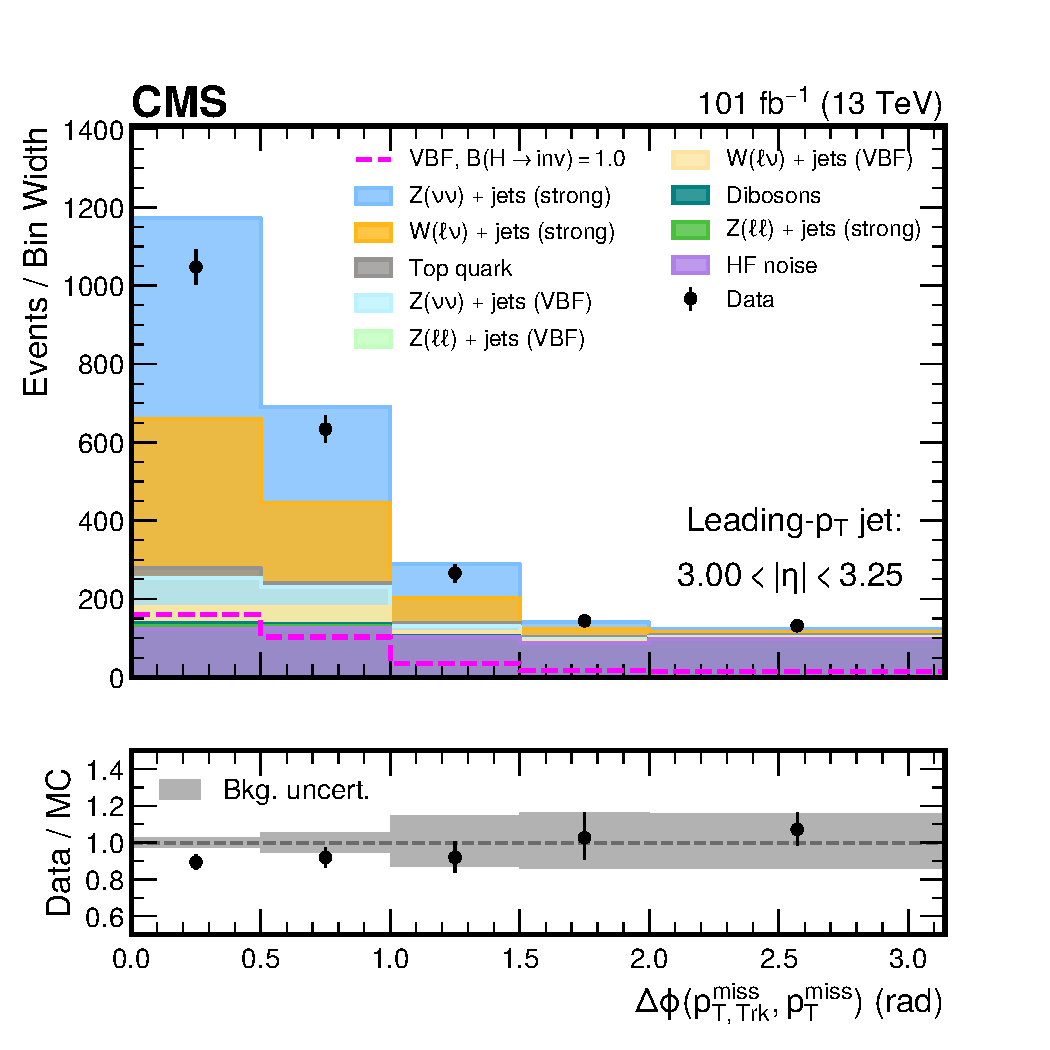
\includegraphics[width=0.7\textwidth]{HFStudy/NoiseEstimation/data_mc_eta_3_3_25_combined.pdf}
    \caption{$\Delta\phi(p_{T,trk}^{miss}, \ptmiss)$ distribution for the closure test on the HF noise estimate. Events plotted here pass the VBF signal 
    region selection, and have the leading jet in $3 < |\eta| < 3.25$ range, where the HF noise contribution is highest.
    It can be observed, especially at high $\Delta\phi(p_{T,trk}^{miss}, \ptmiss)$, the agreement between data and background yields is good
    after the residual HF noise estimation is taken into account. To account for residual differences, a $20\%$ flat uncertainty is assigned to the HF noise template.}
    \label{fig:hf_noise_closure}
\end{figure}

From Fig.~\ref{fig:hf_noise_closure}, it can be observed, especially at high $\Delta\phi(p_{T,trk}^{miss}, \ptmiss)$, the agreement between data and background yields is good
after the residual HF noise estimation is taken into account. To account for residual disagreements between data and background estimation, a $20\%$ flat uncertainty
is assigned to the HF noise template. 

\subsection{Missing HE-15/16 sectors in 2018}
\label{subsec:hem}

During a large part of data-taking in 2018, a submodule of the HCAL was not
functioning. As a result, no HCAL deposits have been recorded in the region of
$-3.0 < \eta < -1.3$ and $-1.57 < \phi < -0.87$ for the affected portion of the
recorded dataset. These missing HCAL deposits have the following consequences
for this analysis:

\begin{itemize}
    \item The jets that are affected will often be wrongly reconstructed as an electron. These mis-reconstructed
    electrons can pass the identification criteria imposed in the electron control regions, due
    to the lack of HCAL energy deposits. Therefore, such events with mis-reconstructed jets in
    this $[\eta,\phi]$ region can contaminate the electron control regions.
    \item Affected jets will not be calibrated correctly, because the energy of the reconstructed jet
    is dependent on all the HCAL deposits. Such mis-calibration will result in anomalous $\ptmiss$ in such events. 
\end{itemize}

Therefore, it was found that the analysis regions that are most impacted by this problem are the signal region and single 
electron control region. Additional requirements were imposed on these two regions to reject mis-reconstructed events arising
due to the missing HCAL deposits. The studies done to identify the impact on the analysis, and the requirements imposed are
outlined below. 

Figure~\ref{fig:HEM_motivation} shows the impact of a veto on 
events having electrons reconstructed in the impacted $[\eta,\phi]$ region. 
The alternative of "ignoring" electrons in that region, i.e. demoting them to jets 
and recalculating the leading jet pair and other relevant selection variables, 
leads to almost identical results: The source of these jets is QCD multijet events, 
hence very few of these events have another good electron to pass the selection for 
$W \rightarrow e \nu$ events. Therefore, an event veto is imposed on the single electron
control region, if the reconstructed electron is found to be within the impacted phase space.

\begin{figure}[htbp]
    \begin{center}
        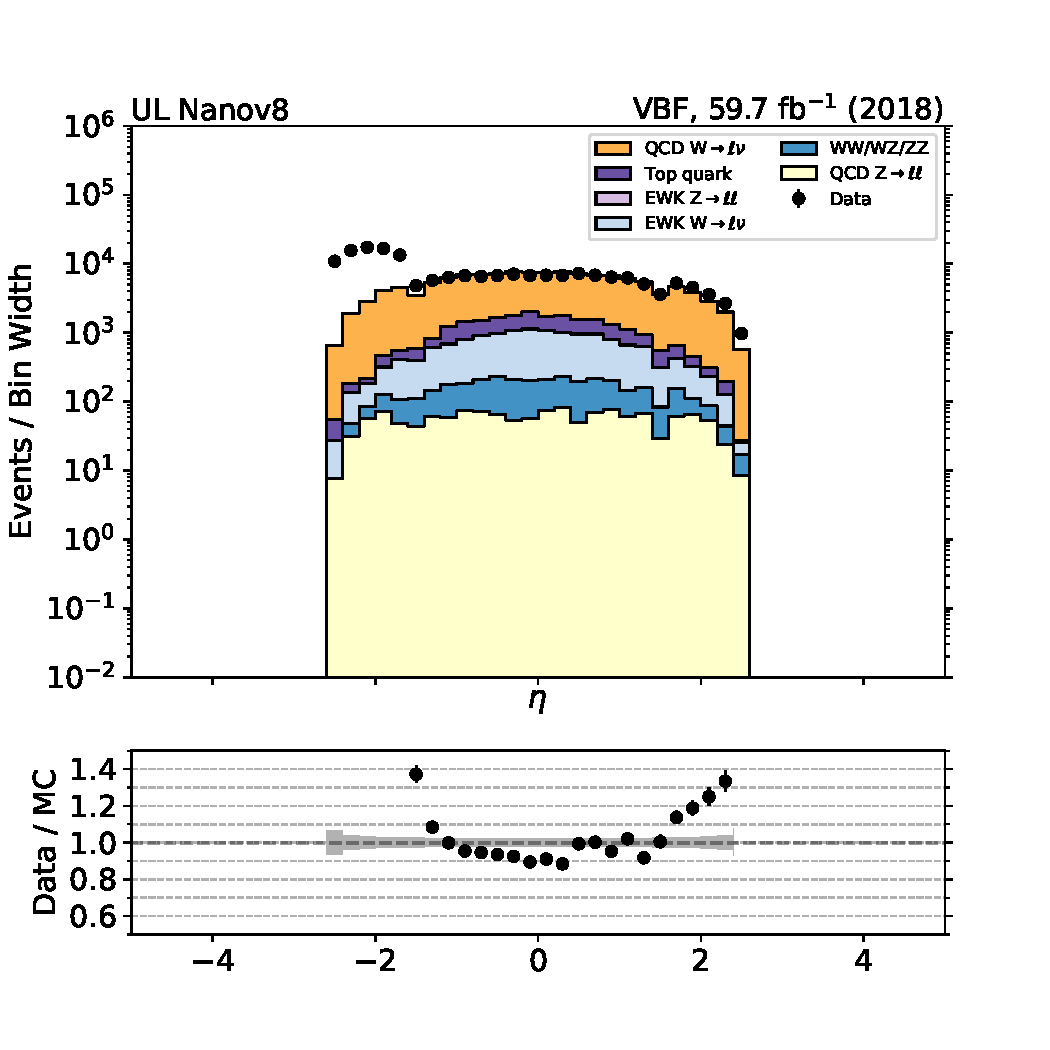
\includegraphics[width=0.49\textwidth]{HEMStudy/cr_1e_vbf_no_hemveto_data_mc_electron_eta_2018.pdf}
        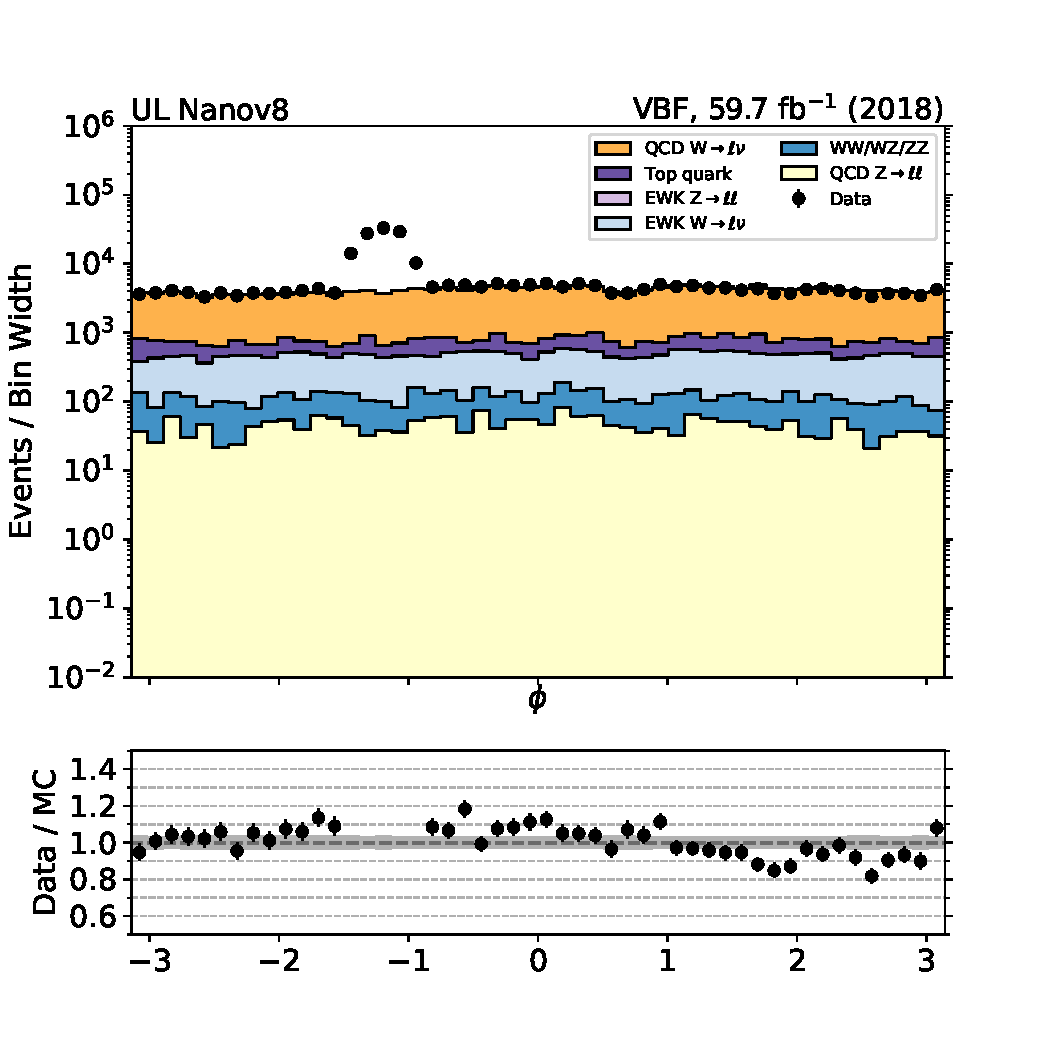
\includegraphics[width=0.49\textwidth]{HEMStudy/cr_1e_vbf_no_hemveto_data_mc_electron_phi_2018.pdf} \\
        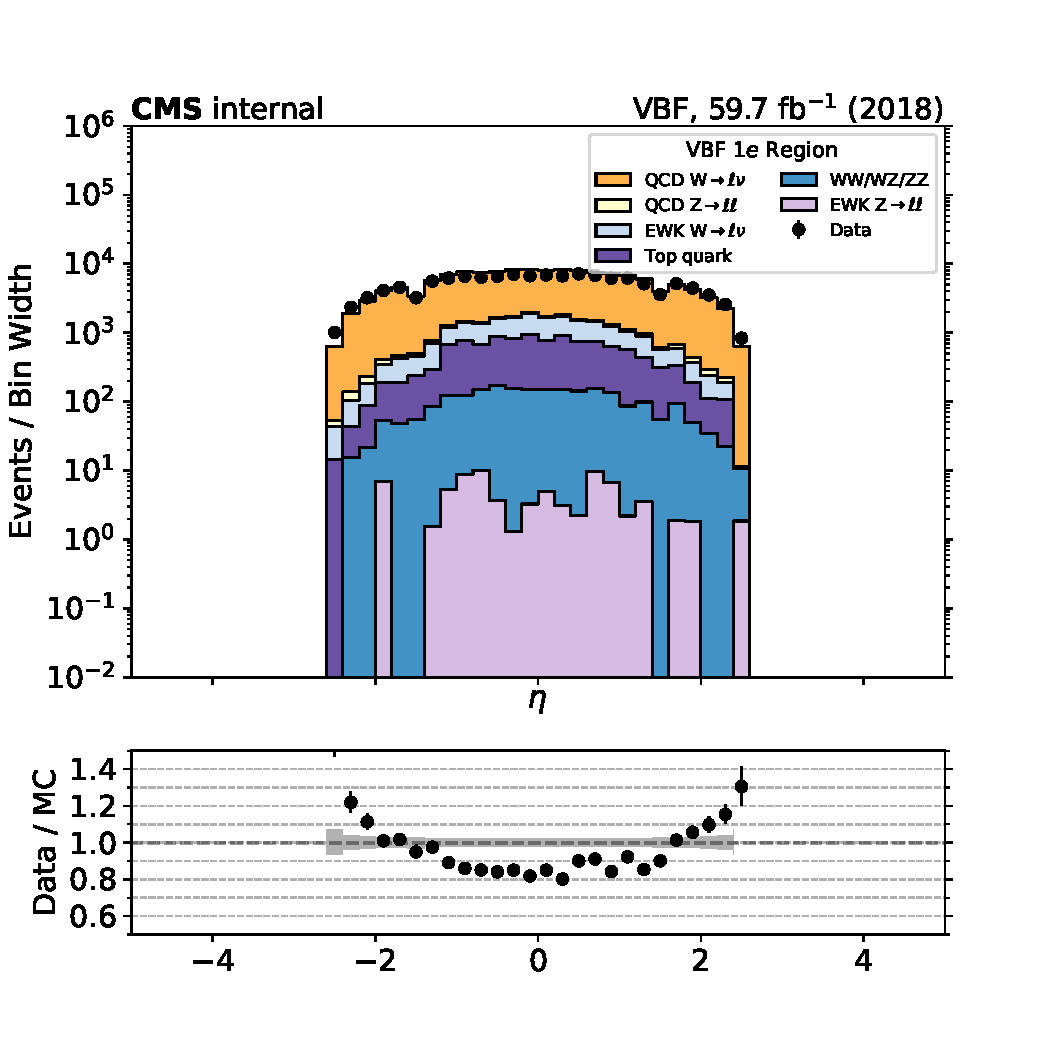
\includegraphics[width=0.49\textwidth]{HEMStudy/cr_1e_vbf_data_mc_electron_eta_2018.pdf}
        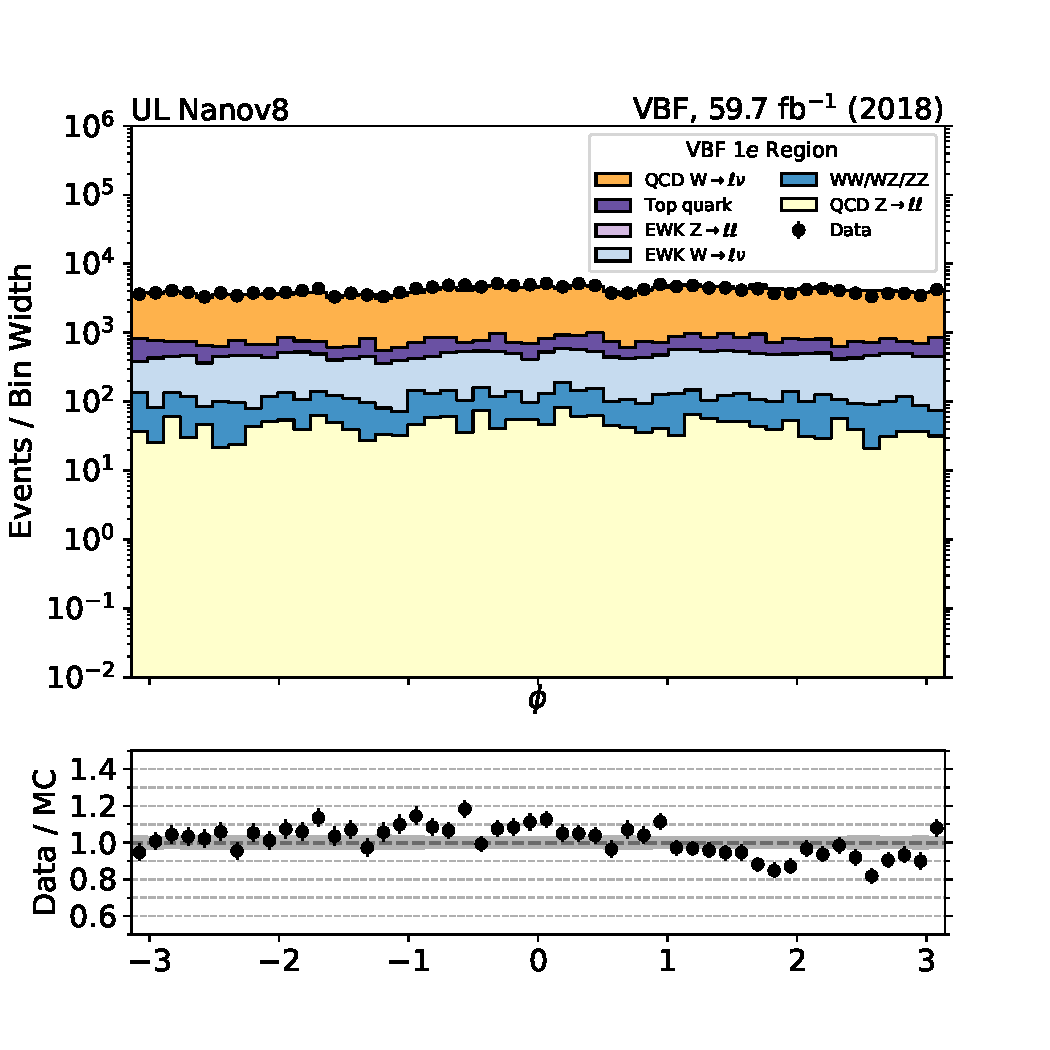
\includegraphics[width=0.49\textwidth]{HEMStudy/cr_1e_vbf_data_mc_electron_phi_2018.pdf}
    \end{center}
    \caption{Effects of an electron veto in the affected detector region (single electron control region 2018). 
    Plots on the top show the $\eta$ and $\phi$ of the highest $\pt$ electron in the event
    without any veto, while plots on the bottom show the $\eta$ and $\phi$ of the electron with the veto.}
    \label{fig:HEM_motivation}
\end{figure}

The muon control regions are not affected from the missing HCAL deposits, 
thanks to the tight muon criteria imposed both in Z and W muon control regions.

The other impacted analysis region is the signal region. 
Figs.~\ref{fig:sr_2018_noHemCut_jetlead} and ~\ref{fig:sr_2018_noHemCut_met} show the distributions, in data and MC, of the leading and subleading 
jet $\phi$ and the $\phi$ of the $\ptmiss$ vector ($\phi_{\ptmiss}$), in the signal region in in 2018. 
From Figs.~\ref{fig:sr_2018_noHemCut_jetlead} and \ref{fig:sr_2018_noHemCut_met}, it can be observed that the agreement between data and MC is good 
except for the region where $-1.8 < \phi_{\ptmiss} < -0.6$. This is co-incident 
with the missing HCAL submodule. The same disagreement can be seen in the jet $\phi$ distributions, on the opposite side in $\phi$, 
which arises due to the signal selection requirement that the jets and missing energy are not aligned.
To mitigate this problem in the signal region, the following additional requirement is imposed on 2018 data:

\begin{itemize}
    \item For events in data where the run number is smaller than 319077 (i.e. before the HCAL submodule malfunctioning)
    no additional requirement is imposed, since those events are not impacted by the problem. Out of the full $59.7 \ fb^{-1}$
    of 2018 data, these events correspond to $21.1 \ fb^{-1}$ of integrated luminosity.
    \item For events in data where the run number is larger or equal to 319077, the event is discarded
    if it has $-1.8 < \phi_{\ptmiss} < -0.6$. These events correspond to a $38.6 \ fb^{-1}$ of integrated luminosity. 
\end{itemize}

The usage of run number to identify if the event is impacted by the missing HCAL submodule allows to keep $100\%$ of the data   
before the problem occurred. This effect is modeled in simulation by reweighting the set of events with $-1.8 < \phi_{\ptmiss} < -0.6$
with the fraction of luminosity without impact. This weight corresponds to $21.1 / 59.7 = 0.35$. Therefore, about $35\%$ of the events
with $-1.8 < \phi_{\ptmiss} < -0.6$ in simulation are kept in the analysis.

\begin{figure}[htbp]
    \begin{center}
        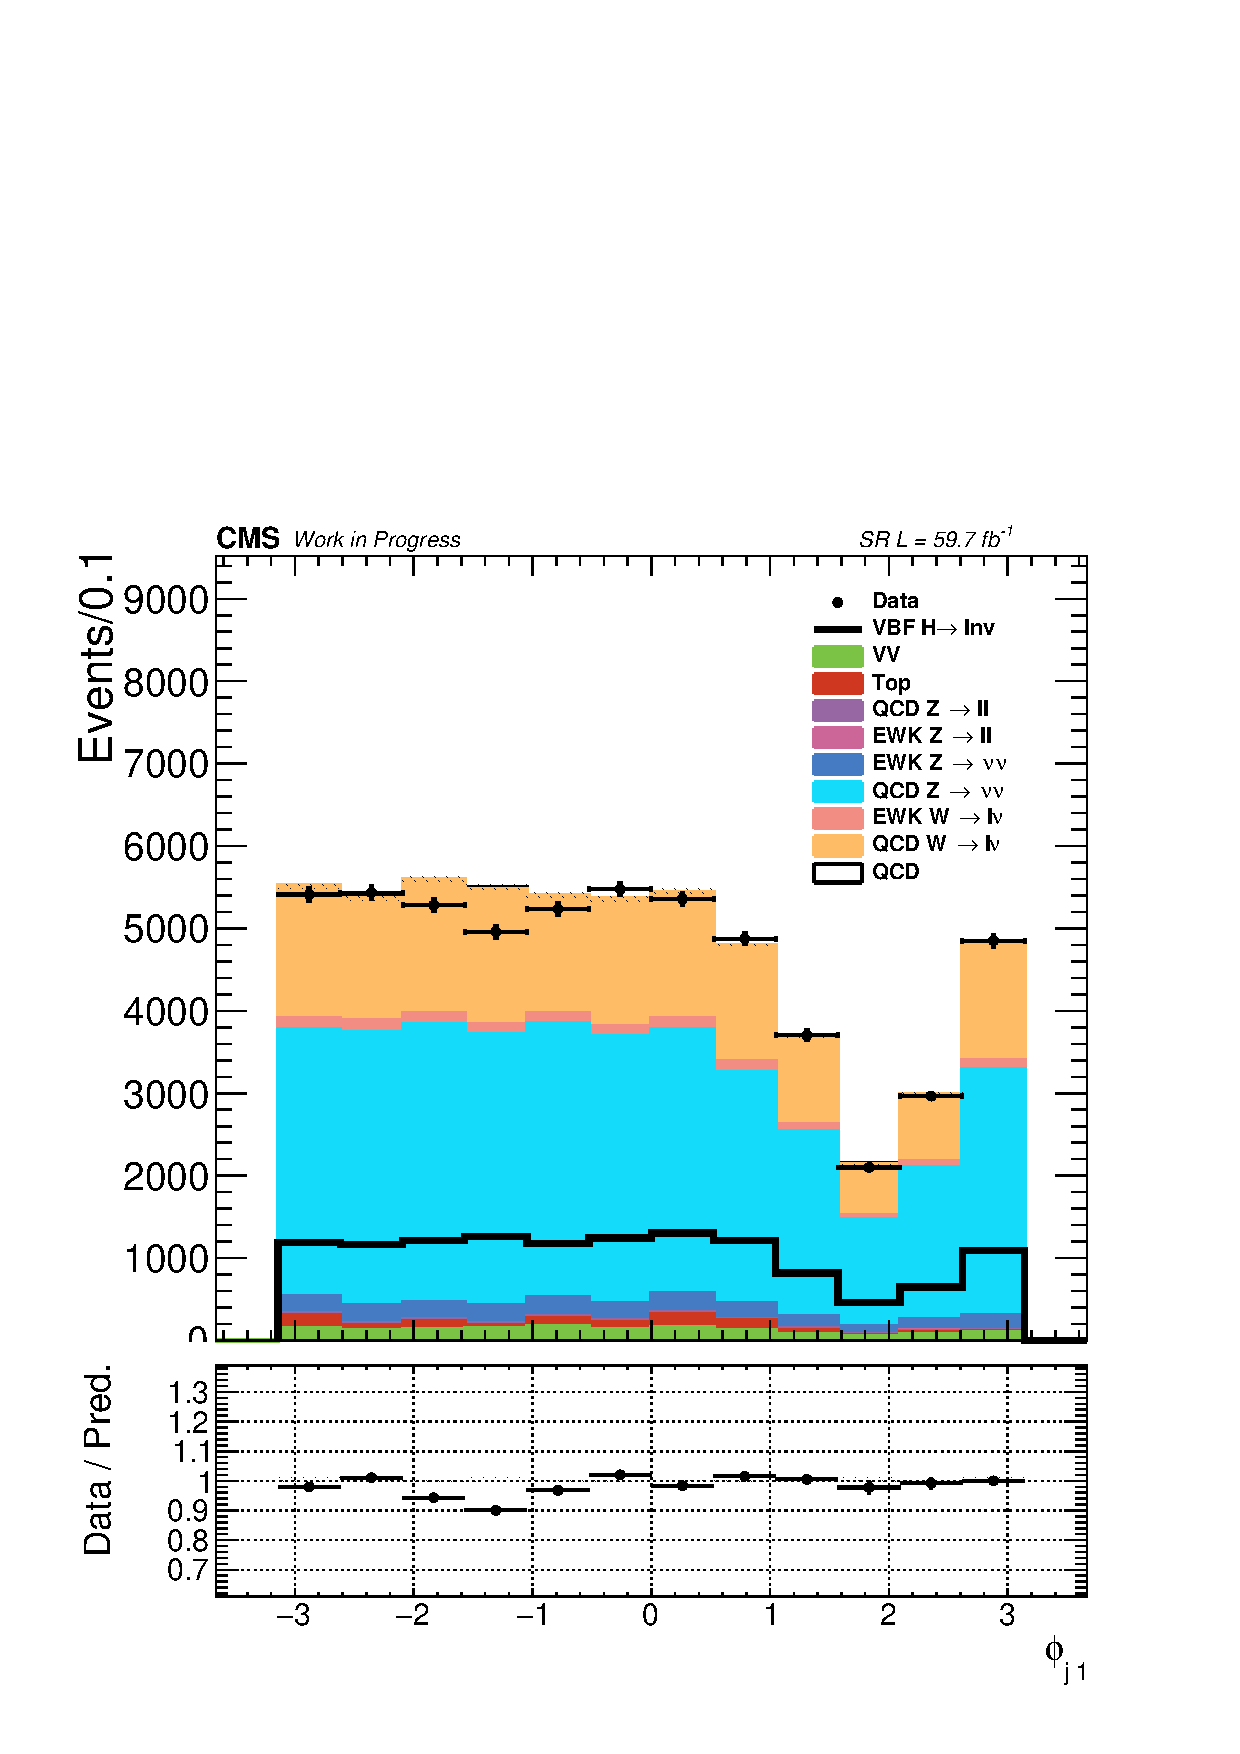
\includegraphics[width=0.49\textwidth]{HEMStudy/Leading_jet_phi.pdf}
        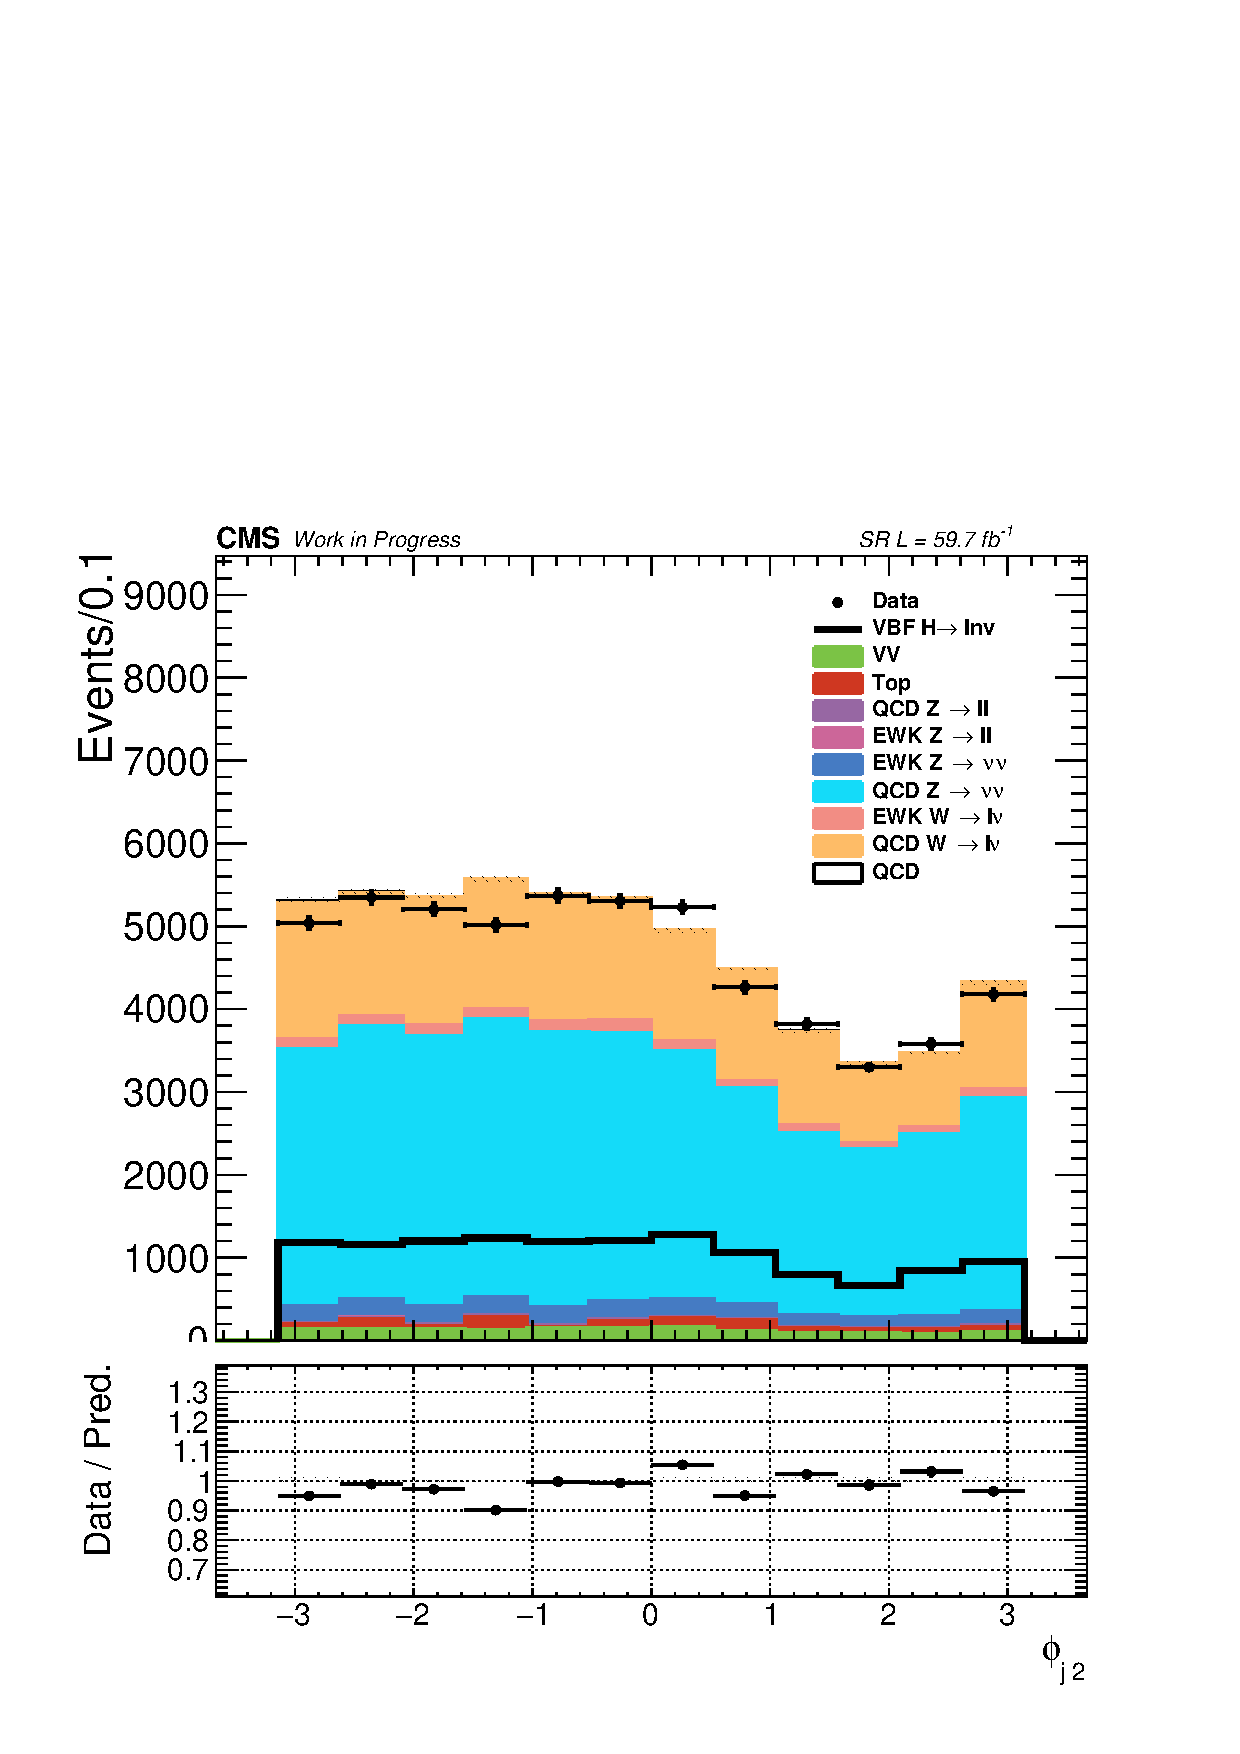
\includegraphics[width=0.49\textwidth]{HEMStudy/Subleading_jet_phi.pdf}
    \end{center}
    \caption{Leading (left) and subleading (right) jet $\phi$ distributions in the signal region from the 2018 dataset.
    The bands in the ratio plots represent the statistical uncertainties in the MC.}
    \label{fig:sr_2018_noHemCut_jetlead}
\end{figure}

\begin{figure}[htbp]
    \begin{center}
        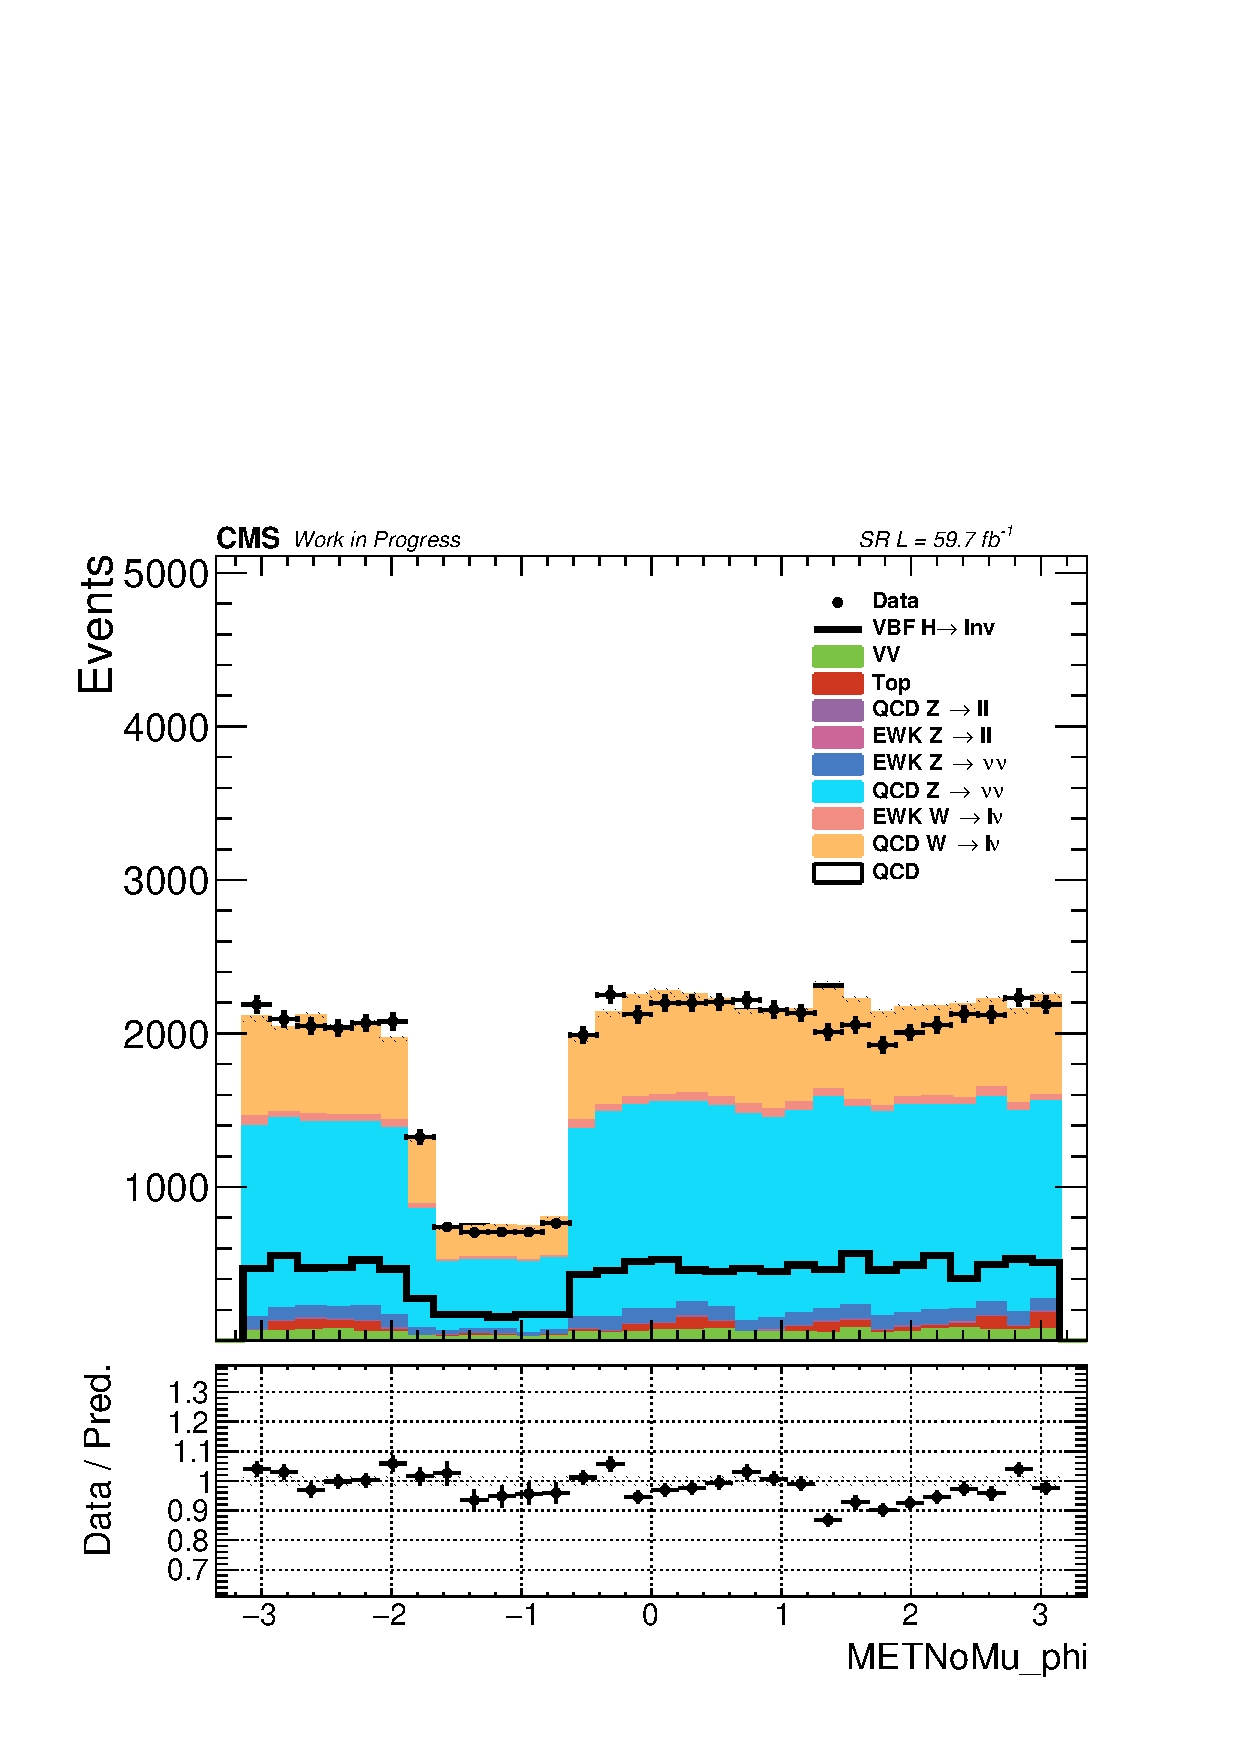
\includegraphics[width=0.7\textwidth]{HEMStudy/MetNoMu_phi.pdf}
    \end{center}
    \caption{$\phi_{\ptmiss}$ distribution in the signal region from the 2018 dataset.}
    \label{fig:sr_2018_noHemCut_met}
\end{figure}

\clearpage